% Format teze zasnovan je na paketu memoir
% http://tug.ctan.org/macros/latex/contrib/memoir/memman.pdf ili
% http://texdoc.net/texmf-dist/doc/latex/memoir/memman.pdf
% 
% Prilikom zadavanja klase memoir, navedenim opcijama se podešava 
% veličina slova (12pt) i jednostrano štampanje (oneside).
% Ove parametre možete menjati samo ako pravite nezvanične verzije
% mastera za privatnu upotrebu (na primer, u b5 varijanti ima smisla 
% smanjiti 
\documentclass[12pt,oneside]{memoir} 

% Paket koji definiše sve specifičnosti master rada Matematičkog fakulteta
\usepackage[latinica]{matfmaster} 
\usepackage{amsthm}

% Podešavanje stila listinga
\usepackage{listings}
\usepackage{xcolor}

\definecolor{codegreen}{rgb}{0,0.6,0}
\definecolor{codegray}{rgb}{0.5,0.5,0.5}
\definecolor{codepurple}{rgb}{0.58,0,0.82}
\definecolor{backcolour}{rgb}{0.95,0.95,0.92}

\lstdefinestyle{mystyle}{
    backgroundcolor=\color{backcolour},   
    commentstyle=\color{codegreen},
    keywordstyle=\color{magenta},
    numberstyle=\tiny\color{codegray},
    stringstyle=\color{codepurple},
    basicstyle=\ttfamily\footnotesize,
    breakatwhitespace=false,         
    breaklines=true,                 
    captionpos=b,                    
    keepspaces=true,                 
    numbers=left,                    
    numbersep=5pt,                  
    showspaces=false,                
    showstringspaces=false,
    showtabs=false,                  
    tabsize=2
}

\lstset{style=mystyle}


\theoremstyle{plain}
\newtheorem{thm}{Teorema}[chapter] % svaki chapter resetuje brojač

\theoremstyle{definition}
\newtheorem{defn}{Definicija} % definicija
\newtheorem{lem}{Lema} % lema
%
% Podrazumevano pismo je ćirilica.
%   Ako koristite pdflatex, a ne xetex, sav latinički tekst na srpskom jeziku
%   treba biti okružen sa \lat{...} ili \begin{latinica}...\end{latinica}.
%
% Opicija [latinica]:
%   ako želite da pišete latiniciom, dodajte opciju "latinica" tj.
%   prethodni paket uključite pomoću: \usepackage[latinica]{matfmaster}.
%   Ako koristite pdflatex, a ne xetex, sav ćirilički tekst treba biti
%   okružen sa \cir{...} ili \begin{cirilica}...\end{cirilica}.
%
% Opcija [biblatex]:
%   ako želite da koristite reference na više jezika i umesto paketa
%   bibtex da koristite BibLaTeX/Biber, dodajte opciju "biblatex" tj.
%   prethodni paket uključite pomoću: \usepackage[biblatex]{matfmaster}
%
% Opcija [b5paper]:
%   ako želite da napravite verziju teze u manjem (b5) formatu, navedite
%   opciju "b5paper", tj. prethodni paket uključite pomoću: 
%   \usepackage[b5paper]{matfmaster}. Tada ima smisla razmisliti o promeni
%   veličine slova (izmenom opcije 12pt na 11pt u \documentclass{memoir}).
%
% Naravno, opcije je moguće kombinovati.
% Npr. \usepackage[b5paper,biblatex]{matfmaster}

% Pomoćni paket koji generiše nasumičan tekst u kojem se javljaju sva slova
% azbuke (nema potrebe koristiti ovo u pravim disertacijama)

% Datoteka sa literaturom u BibTex tj. BibLaTeX/Biber formatu
\bib{literatura}

% Ime kandidata na srpskom jeziku (u odabranom pismu)
\autor{Lazar S. Mladenović}
% Naslov teze na srpskom jeziku (u odabranom pismu)
\naslov{Automatsko ispravljanje grešaka detektovanih pomoću alata Memcheck }
% Godina u kojoj je teza predana komisiji
\godina{2020}
% Ime i afilijacija mentora (u odabranom pismu)
\mentor{doc. dr Milena \textsc{Vujošević Janičić}, docent \\ Univerzitet u Beogradu, Matematički fakultet}
% Ime i afilijacija prvog člana komisije (u odabranom pismu)
\komisijaA{prof. dr Miodrag \textsc{Živković}, redovan profesor\\ Univerzitet u Beogradu, Matematički fakultet}
% Ime i afilijacija drugog člana komisije (u odabranom pismu)
\komisijaB{prof. dr Filip \textsc{Marić}, vanredni profesor\\ Univerzitet u Beogradu, Matematički fakultet}
% Ime i afilijacija trećeg člana komisije (opciono)
% \komisijaC{}
% Ime i afilijacija četvrtog člana komisije (opciono)
% \komisijaD{}
% Datum odbrane (odkomentarisati narednu liniju i upisati datum odbrane ako je poznat)
 \datumodbrane{}

% Apstrakt na srpskom jeziku (u odabranom pismu)
\apstr{
Verifikacija softvera zauzima bitno mesto u procesu razvoja softvera. Dinamička verifikacija softvera zasniva se na proveri ispravnosti softvera koja se vrši tokom njegovog izvršavanja. Postoje razni alati i platforme za dinamičku verifikaciju softvera, a jedna značajna platforma je \textit{Valgrind}. Alati njegove distribucije mogu dati profile programa koji mogu pomoći u poboljšanju rada i performansa programa, a takođe mogu i ukazati na greške u okviru programa koje nije lako otkriti. Važan alat platforme \textit{Valgrind} je \textit{Memcheck}. Ovaj alat analizira i ukazuje na greške u radu sa memorijom. Te greške mogu da izazovu pad programa, a uključuju, na primer, korišćenje neinicijalizovane vrednosti i pristup oslobođenoj, odnosno nedozvoljenoj memoriji. Cilj ovog rada je konstrukcija alata koji će koristeći izvešataj koji daje \textit{Valgrind}, odnosno \textit{Memcheck}, otkriti i ispraviti uzroke grešaka u programu. Osnovna ideja za ostvarivanje ovog cilja je da se definišu relevantni šabloni za ispravljanje grešaka i da se implementira automatska analiza izveštaja koji se dobija iz alata \textit{Memcheck} i koja korišćenjem odgovarajućih šablona postiže željenu funkcionalnost. 
}

% Ključne reči na srpskom jeziku (u odabranom pismu)
\kljucnereci{Verifikacija softvera, dinamička analiza, profajliranje, Valgrind, Memcheck}

\begin{document}
% ==============================================================================
% Uvodni deo teze
\frontmatter
% ==============================================================================
% Naslovna strana
\naslovna
% Strana sa podacima o mentoru i članovima komisije
\komisija
% Strana sa posvetom (u odabranom pismu)
\posveta{Familiji}
% Strana sa podacima o disertaciji na srpskom jeziku
\apstrakt
% Sadržaj teze
\tableofcontents*

% ==============================================================================
% Glavni deo teze
\mainmatter
% ==============================================================================

% ------------------------------------------------------------------------------
\chapter{Uvod}
% ------------------------------------------------------------------------------
Razvoj softvera predstavlja složen proces koji obuhvata razne aktivnosti. Nepisano je pravilo da se prilikom pisanja programa može desiti da se provuče neka greška kao npr. neinicijalizacija promenljive, ili neoslobađanje alocirane memorije, koja u tom trenutku možda biva bezazlena. Međutim, kako razvoj programa odmiče, dodatne greške koje ta početna, naizgled bezazlena greška izaziva, bivaju krucijalne i od vitalnog značaja. Na neke od gore pomenutih grešaka, nažalost kompliator ne može da nam ukaže. Ovo nije veliki problem ukoliko su naši programi mali, ali u  kompleksnijim programima, onim koji se sastoje od više hiljada linija koda, greške je teško naći. 

Verifikacija softvera ima za cilj ispravljanje tih grešaka i zauzima bitno mesto u procesu razvoja softvera. Statička verifikacija softvera analizira ispravnost programa bez njegovog izvršavanja, tj.~vrši analizu izvornog koda, dok dinamička verifikacija softvera predstavlja tehniku ispitivanja ispravnosti koda u toku njegovog izvršavanja \cite{02Motivacija}. Binarna analiza obuhvata analizu na nivou mašinskog koda, snimljenog kao objektni k\^od (nepovezan) ili kao izvršni k\^od (povezan) \cite{03DinamickaAnaliza}. Primer platforme koji vrši dinamičku binarnu analizu koda jeste \textit{Valgrind}.  

\textit{Valgrind} je platforma koja pruža brojne alate za debagovanje i profajliranje koji pomažu da se brže i pravilnije otklone greške u programima. Najpopularniji od ovih alata zove se \textit{Memcheck}. Ovaj alat može otkriti mnoge greške u vezi sa memorijom koje su česte u programima C i C++, a koje mogu dovesti do pada ili nepredvidivog ponašanja programa. 

Platforma \textit{Valgrind} sa svim svojim alatima samo ukazuje na greške, kao i na to šta ih je izazvalo. Ispravljanje istih ostaje programeru. Cilj ovog rada jeste da automatizuje ispravljanje grešaka na koje ukazuje alat \textit{Valgrind}, tako što će koristiti precizno definisane šablone za ispravljanje grešaka. U realizaciji te ideje će se primenjivati regularni izrazi kojima će biti opisani izrazi koji mogu da prouzrokuju greške na koje nam ukazuje \textit{Memcheck}.

U glavi 2 platforma \textit{Valgrind} će biti detaljno opisana. Biće pobrojani i obrađeni svi alati \textit{Valgrind}-a. Najveći akcenat će biti na alatu \textit{Memcheck}, dok će o ostalima biti date osnovne relevantne informacije. U glavi 3 biće ukratko reči o procesu kompilacije programa i njenim fazama. Centralno mesto zauzeće teorija o jezicima i regularnim izrazima. U glavi 4 biće predstavljen alat \textit{Koronka}, koji je osnovni doprinos ovog rada: biće opisana arhitektura, algoritam izvršavanja i njegove funkcionalnosti. Takođe, čitaoci će biti bliže upoznati sa načinom upotrebe i rada alata. Na kraju, biće iznet osvrt na ceo rad. Kako tema to afirmiše, a i sam alat je napravljen tako da može da se stalno unapređuje, u smislu uopštavanja postojećih šablona, primene drugih vrsta analiza i alata \textit{Valgrind}-a i sl., biće iznete i ideje i mogućnosti za dalji razvoj ovog projekta.


\chapter{Alat Valgrind}
\textit{Valgrind}\footnote{ Ime \textit{Valgrind} potiče iz nordijske mitologije.} je platforma za pravljenje alata za dinamičku analizu \cite{Valgrind}. Dolazi sa skupom alata, od kojih svaki obavlja neku vrstu debagovanja, profajliranja ili slične zadatke koji pomažu programeru da poboljša program koji razvija. \textit{Valgrind} se može koristiti i kao alat za pravljenje novih alata, bez narušavanja postojeće strukture. 
\textit{Valgrind} distribucija trenutno broji sledeće alate:
\begin{enumerate}
  \item \textit{Memcheck} \cite{Memcheck} --- alat za detekciju memorijskih grešaka.
  \item \textit{Cachegrind}  \cite{Cachegrind} --- profajler keš memorije i skokova. 
  \item \textit{Callgrind} \cite{Callgrind} --- profajler poziva funkcija. % Ima nekih preklapanja sa \textit{Cachegrind} - om, ali takođe pruža neke informacije koje \textit{Cachegrind} ne.
  \item \textit{Helgrind} \cite{Helgrind} --- alat za detekciju grešaka niti.
  \item \textit{DRD} \cite{Drd} --- takođe alat za detekciju grešaka niti. % Sličan je \textit{Helgrind}-u, ali koristi različite tehnike analize i tako može naći različite probleme.
  \item \textit{Massif} \cite{Massif} --- profajler korišćenja dinamičke memorije.
  \item \textit{DHAT} \cite{DHAT} --- profajler korišćenja dinamičke memorije. % predstavlja drugu vrstu profajlera hipa koji pomaže u razumevanju problema sa životnim vekom bloka, upotrebom bloka i neefikasnošću rasporeda.
  \item \textit{BBV} \cite{BBV} --- eksperimentalni alat za podršku razvoja novih arhitektura računara. % eksperimentalni alat za generisanje osnovnih vektorskih blokova za dalju analizu \textit{SimPoint} altima, koji je u mnogome korisntan ljudima koji se bave istraživanjem i razvojem računarske arhitekture.
\end{enumerate}
Platforma \textit{Valgrind} radi na sledećim arhitekrurama:
\begin{itemize}
  \item Linux: x86, AMD64, ARM, ARM64, PPC32, PPC64, PPC64LE, S390X, MIPS32, MIPS64.
  \item Solaris: x86, AMD64. 
  \item Android: ARM (2.3.x i novije), ARM64, x86 (4.0 i novije), MIPS32 
  \item Darwin: x86, AMD64 (Mac OS X 10.12)\cite{Valgrind}
\end{itemize}

\section{Arhitektura i princip funkcionisanja}
Arhitekturu alata \textit{Valgrind} možemo najjednostavnije opisati pomoću formule:
\begin{center}
\texttt{jezgro Valgrind-a + alat koji se dodaje = alat Valgrind-a}.
\end{center}

Jezgro \textit{Valgrind}-a omogućava izvršavanje klijentskog programa, kao i snimanje izveštaja koji su nastali prilikom analize samog programa. Alat za dinamičku analizu koda se kreira kao dodatak na jezgro \textit{Valgrind}-a, pisan u programskom jeziku C.

Alati \textit{Valgrind}-a koriste metodu bojenja vrednosti. Princip funkcionisanja je takav da svaki registar i memorijsku vrednost ''boje'' (zamenjuju) sa vrednošću koja govori nešto dodatno o originalnoj vrednosti.

Svi \textit{Valgrind} alati rade na istoj osnovi, s tim da informacije koje se emituju variraju. Te informacije mogu se iskoristiti za otklanjanje grešaka, optimizaciju koda ili bilo koju drugu svrhu za koju je alat dizajniran.

Sledeća komanda ilustruje način pokretanja alata Valgrind:
\begin{center}
\texttt{valgrind --tool=alat [argumenti alata] ./izvršniProgram [argumenti izvršnog programa]}.
\end{center}

Svaki \textit{Valgrind}-ov alat je statički povezana izvršna datoteka koja sadrži k\^od alata i k\^od jezgra. Izvršna datoteka \textit{valgrind} predstavlja program omotač koji na osnovu \texttt{--tool} opcije bira alat koji treba pokrenuti. Sem opcije \texttt{--tool} postoji mnoštvo opcija koje precizno definišu rad \textit{Valgrind} alata, kao npr.:
\begin{itemize}
\item \texttt{--track-origins} koja daje bliže informacije i detaljniji izveštaj o greškama koje su izazvane, 
\item \texttt{--leack-check} koja svako curenje memorije prikazuje detaljnjno,
\item \texttt{--show-leack-kinds} koja prikazuje sve vrste curenja koje su definitivne, indirektne, moguće i dostupne u celom izveštaju,
\item \texttt{--log-file}  koja će izlaz alata \textit{Valgrind} proslediti u navedenu datoteku (podrazumevano \textit{Valgrind} svoj izlaz ispisuje na terminal).
\end{itemize} 
Sve ove komande će biti detaljnije objašnjene u sekcijama koje slede. Naredni primer ilustruje pokretanje \textit{Valgrind}-a sa dodatnim argumentima.
\begin{center}
\texttt{valgrind --track-origins=yes --leack-check=full --show-leak-kinds=all --log-file=LOG.txt ./a.out}.
\end{center}
Podrazumevani alat je \textit{Memchek}, tako da se u navedenom gore poziva alat \textit{Memchek} nad izvršnim programom \textit{a.out}.

Izvršna datoteka alata statički je linkovana tako da se učitava počev od neke adrese koja je obično dosta iznad adresnog prostora koji koriste klasičan korisnički program (na \textit{x86/Linux} i \textit{MIPS/Linux} koristi se adresa 0x38000000). \textit{Valgrind}-ovo jezgro prvo inicijalizuje podsistem kao što su menadžer adresnog prostora i njegov unutrašnji alokator memorije, a zatim učitava klijentovu izvršnu datoteku. Potom se inicijalizuju \textit{Valgrind}-ovi podsistemi kao što su translaciona tabela, aparat za obradu signala, raspoređivač niti i učitavaju se informacije za debagovanje klijenta, ukoliko postoje. Od tog trenutka \textit{Valgrind} ima potpunu kontrolu i počinje sa prevođenjem i izvršavanjem klijentskog programa. Može se reći da \textit{Valgrind} vrši \textit{JIT (Just In Time)} kompajliranje mašinskog koda programa u mašinski k\^od programa dopunjen instrumentacijom. Time se postiže da se nijedan deo koda klijenta ne izvršava u svom izvornom obliku. To funkcioniše tako što alat u originalni k\^od umeće operacije u svrhu instrumentacije, zatim se takav k\^od prevodi. Proces prevođenja se sastoji iz raščlanjivanja originalnog mašinskog koda u odgovarajuću međureprezentaciju (eng. \textit{intermediate representation}, skraćeno IR) koji se kasnije instrumentalizuje sa alatom i ponovo prevodi u novi mašinski k\^od.

Rezultat svega ovoga se naziva translacija, koja se čuva u memoriji i koja se izvršava po potrebi. Jezgro troši najviše vremana na sam proces pravljenja,  pronalaženja i izvršavanja translacije. Jedini problem koji se ovde može dogoditi je ako se vrši translacija koda koji se menja tokom izvršavanja programa.

Postoje mnoge komplikacije koje nastaju prilikom smeštanja dva programa u jedan proces (klijentski program i program alata). Mnogi resursi se dele između ova dva programa, kao što su registri ili memorija. Takođe, alat \textit{Valgrind}-a ne sme da se odrekne totalne kontrole nad izvršavanjem klijentskog programa prilikom izvršavanja sistemskih poziva, signala i niti.

\subsection*{Osnovni blok}
\textit{Valgrind} deli originalni k\^od u sekvence koje se nazivaju osnovni blokovi. Osnovni blok je pravolinijska sekvenca mašinskog koda, na čiji se početak skače, a koja se završava sa skokom, pozivom funkcije ili povratkom u funkciju pozivaoca. Svaki k\^od programa koji se analizira ponovo se prevodi na zahtev, pojedinačno po osnovnim blokovima, neposredno pre samog izvršavanja samog bloka. Ako uzmemo da su osnovni blokovi klijentskog koda OB1, OB2, ...~, onda prevedene osnovne blokove obeležavamo sa t(OB1), t(OB2), itd.. Veličina osnovnog bloka je ograničena na maksimalno šezdeset mašinskih instrukcija.

\subsection*{Sistemski pozivi}
Usluge koje operativni sistem može da pruži aplikativnim programima realizuju se pomoću sistemskih poziva (eng. \textit{system calls}). Programi uz pomoć sistemskih poziva komuniciraju sa jezgrom operativnog sistema i pomoću njega dobijaju mogućnost da izvrše osetljive operaciju u sistemu. Praktično, sistemski pozivi su skup funkcija koji predstavlja interfejs ka operativnom sistemu. 

Procesori savremenih računarskih sistema imaju mogućnost rada u dva režima – korisničkom (eng. \textit{user mode}) i sistemskom (eng. \textit{supervisor, kernel mode}). U sistemskom režimu moguće je izvršiti sve instrukcije, dok je broj instrukcija koje možemo izvršiti u korisničkom redukovan. Naime, instrukcije za osetljive operacije poput pristupa U/I uređajima, zaštićenim delovima memorije itd., moguće je izvršiti samo u sistemskom režimu rada procesora. Aplikativni programi se veći deo vremena izvršavaju u korisničkom režimu, dok je sistemski režim, kao što je već napomenuto, zadužen za posebno osetljive operacije koje izvodi operativni sistem. Pri korišćenju sistemskog poziva prelazi se iz korisničkog u sistemski režim, a dalju kontrolu preuzima operativni sistem. Ključni deo operativnog sistema koji reaguje u ovakvim situacijama je jezgro operativnog sistema.

Sistemski pozivi se realizuju pomoću sistema prekida.  Korisnički program postavlja parametre sistemskog poziva na određene memorijske lokacije ili registre procesora, inicira prekid, operativni sistem preuzima kontrolu, uzima parametre, izvršava tražene radnje, rezultat stavlja na određene memorijske lokacije ili u registre i vraća kontrolu korisničkom programu.

Nakon svega, zaključujemo da sistemski pozivi obezbeđuju spregu između programa koji se izvršava i operatvinog sistema. Generalno, realizuju se na asemblerskom jeziku, ali viši prograsmki jezici, poput jezika C i C++, takođe omogućavaju realizaciju sistemskih poziva. Program koji se izvršava može proslediti parametre oprativnom sistemu na više načina. Jedan način je prosleđivanje parametara preko registara procesora. Drugi način je  postavljnje parametara u tabelu u memoriji, pri čemu se adresa tabele prosleđuje u registru procesora, postavljanjem parametara na vrh steka (eng. \textit{push}), koje operatvni sistem ''skida'' (eng. \textit{pop}).

Sistemski pozivi se izvršavaju bez posredstva \textit{Valgrind}-a, zato što jezgro \textit{Valgrind}-a ne može da prati njihovo izvršavanje u samom jezgru operativnog sistema \cite{os}. 

\subsection*{Translacije}
U nastavku su opisani koraci kroz koje \textit{Valgrind} prolazi prilikom analize programa. Postoji osam faza translacije. Sve faze osim instrumentacije obavlja jezgro \textit{Valgrind}-a. Instrumentaciju obavlja alat \textit{Valgrind}-a.
\begin{enumerate}
\item \textit{Disasembliranje (razgradnja)} - prevođenje mašinskog koda u ekvivalentni interni skup instrukcija koje se nazivaju međukod instrukcije. U ovoj fazi međukod je predstavljen stablom. Ova faza je zavisna od arhitekture na kojoj se izvršava. 
\item \textit{Optimizacija 1} - prva faza optimizacije linearizuje prethodno izgrađeni međukod. Primenjuju se neke standardne optimizacije programskih prevodilaca kao što su uklanjanje redudantnog koda i eliminacija podizraza.
\item \textit{Instrumentacija} - blok međukoda se prosleđuje alatu, koji može proizvoljno da ga transformiše. Prilikom instrumentacije alat u zadati blok dodaje dodatne međukod operacije, kojima proverava ispravnost rada programa. Treba napomenuti da ubačene instrukcije ne smeju da narušavaju konzistentno izvršavanje originalnog koda. 
\item \textit{Optimizacija 2} - jednostavnija faza optimizacije od prve. Uključuje izračunavanje matematičkih izraza koji se mogu izvršiti pre faze izvršavanja i uklanjanje mrtvog koda.
\item \textit{Izgradnja stabla} - linearizovani međukod se konvertuje natrag u stablo radi lakšeg izbora instrukcija. 
\item \textit{Odabir instrukcija} - Stablo međukoda se konvertuje u listu instrukcija koje koriste virtualne registre. Ova faza se takođe razlikuje u zavisnosti od arhitetkure na kojoj se izvršava. 
\item \textit{Alokacija registara} - zamena virtualnih registara stvarnim. Po potrebi se uvode prebacivanja u memoriju. Koristi se poziv funkcija koje pronalaze iz kojih se registara vrši čitanje i u koje se vrši upis.
\item \textit{Asembliranje} - kodiranje izabranih instrukcija na odgovarajući način i smeštaju u blok memorije. Ova faza se takode razlikuje u zavisnosti od arhitekture na koji se izršava \cite{03DinamickaAnaliza,AKMSc}. 
\end{enumerate}

Kada koristite \textit{Valgrind} alate, bilo bi korisno ponovo kompajlirati aplikaciju i podržati biblioteke sa omogućenim informacijama o otklanjanju grešaka (opcija \texttt{-g}). Bez ovih informacija, najbolje što će \textit{Valgrind}-ovi alati  moći da urade je da pogode kojoj funkciji pripada određeni komad koda, što čini i poruke o greškama i profajliranje rezultata gotovo beskorisnim. Pomoću opcije \texttt{-g} dobićete poruke koje vode direktno do odgovarajuće linije izvornog koda \cite{ValgrindCore}.

\section{Prijavljivanje grešaka}
Alati \textit{Valgrind}-a pišu komentare koji sadrže detaljne izveštaje o greškama i drugim značajnim događajima. Svi redovi u komentaru imaju sledeći oblik:
\begin{center}
\texttt{==12345== odgovarajuća-poruka-alata-Valgrind}.
\end{center}
12345 je ID procesa. Ova šema olakšava razlikovanje izlaznih rezultata programa od komentara \textit{Valgrind}-a, a takođe i razlikovanje komentara od različitih procesa koji su se spojili iz bilo kog razloga.

\textit{Valgrind}-ovi alati podrazumevano pišu u komentar samo ključne poruke, kako bi izbegli da vas preplave informacijama od sekundarne važnosti. Ako želite više informacija o tome šta se događa, pokrenite ponovo \textit{Valgrind} uz opciju \texttt{–v}.

Kada alat za proveru greške otkrije da se nešto loše događa u programu, u komentar se upisuje poruka o grešci. Na slici \ref{fig:slika2.1} prikazan je izlaz iz alata \textit{Memcheck}.
\begin{figure}[!ht]
  \centering
  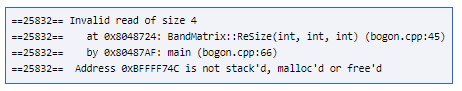
\includegraphics[width=0.8\textwidth]{errorReporting.png}
  \caption{Primer izlaza alta Memcheck, izvor: \cite{ValgrindCore}}
  \label{fig:slika2.1}
\end{figure}

Ova poruka kaže da je program izvršio ilegalno 4-bajtno čitanje adrese 0xBFFFF74C, koja, koliko \textit{Memcheck} može reći, nije važeća adresa steka niti odgovara bilo kojem trenutnom bloku hipa ili nedavno oslobođenim blokovima hipa. Čitanje se događa u redu 45 \textit{bogon.cpp}, pozvanog iz reda 66 iste datoteke. Za greške povezane sa identifikovanim (trenutnim ili oslobođenim) blokom hipa, npr. čitanje oslobođene memorije, \textit{Valgrind} izveštava ne samo o lokaciji na kojoj se dogodila greška, već i gde je pridruženi blok hipa dodeljen/oslobođen.

\textit{Valgrind} pamti sve izveštaje o greškama. Kada se otkrije greška, ona se upoređuje sa starim izveštajima da bi se videlo da li je duplikat. Ako je tako, greška je zabeležena, ali dalji komentari se ne emituju. Na ovaj način, alat izbegava zatrpavanje milionima duplikata izveštaja o greškama.  

Zanimljivo je da se greške prijavljuju pre nego što se pridružena operacija zaista dogodi. Na primer, ako koristite \textit{Memcheck} i vaš program pokušava da čita sa adrese nula, \textit{Memcheck} će poslati poruku u tom smislu, a vaš program će onda verovatno pući sa greškom \textit{Segmentation fault}. Generalno, dobra je praksa ispravljati greške redosledom u kojem su prijavljene. Ukoliko se ne primeni pomenuta praksa, to može da zbuni. Na primer, program koji kopira neinicijalizovane vrednosti na nekoliko memorijskih lokacija i kasnije ih koristi, generisaće nekoliko poruka o grešci kada se pokrene na \textit{Memcheck}-u. Prva takva poruka o grešci može sasvim direktno dati osnovni uzrok problema. 

Proces otkrivanja duplikata grešaka prilično je skup i može prouzrokovati značajno usporenje ako program generiše ogromne količine grešaka. Da bi izbegao ozbiljnije probleme, \textit{Valgrind} će jednostavno zaustaviti prikupljanje grešaka nakon što uoči 1.000 različitih grešaka ili ukupno 10.000.000 grešaka. U ovoj situaciji možete zaustaviti program i popraviti ga, jer \textit{Valgrind} neće reći ništa drugo korisno nakon ovoga. Imajte na umu da se ograničenja od 1.000 / 10.000.000 primenjuju nakon uklanjanja potisnutih grešaka, odnosno onih grešaka za koje \textit{Memcheck} utvrdi da su duplikati. Ova ograničenja su definisana u \textit{m\_errormgr.c} i mogu se povećati ako je potrebno \cite{ValgrindCore}. 

\section{Memcheck}
\textit{Memcheck} je detektor grešaka u memoriji. Kako vrši analizu nad mašinskim, a ne nad izvornim kodom, \textit{Memcheck} ima mogućnost analize programa pisanih u bilo kom jeziku. Može da otkrije sledeće probleme koji su česti u programima C i C ++:
\begin{itemize}
\item Pristup memoriji kojoj ne biste smeli, tj.~prekoračenje i potkopavanje blokova hipa, prekoračenje vrha steka i pristup memoriji nakon što se oslobodi.
\item Korišćenje nedefinisanih vrednosti, tj.~vrednosti koje nisu inicijalizovane ili su izvedene iz drugih nedefinisanih vrednosti.
\item Pogrešno oslobađanje hip memorije, poput dvostrukog oslobađanja blokova hipa, ili neusklađena upotreba \textit{malloc/new/new[]} naspram \textit{free/ delete/delete[]}.
\item Preklapanje \textit{src} i \textit{dst} pokazivača u \textit{memcpy} i srodnim funkcijama.
\item Prosleđivanje sumnjive (verovatno negativne) vrednosti parametru veličine funkcije dodeljivanja memorije.
\item Curenje memorije.
\end{itemize}

Problemi poput ovih teško se mogu pronaći drugim sredstvima, često ostajući neotkriveni tokom dužih perioda, a zatim uzrokujući povremene, teško dijagnostikovane padove. Upravo iz tih razloga memorijske greške spadaju u grupu najteže detektujućih grešaka pa je samim tim i njihovo otklanjanje težak zadatak.

Kao što je rečeno u prethodnoj sekciji, da bi uspešno analizirali program koristeći \textit{Memcheck}, program kompajliramo sa uključenom opcijom \texttt{-g}. Što se optimizacije tiče, prilikom korišćenja alata \textit{Memcheck}, u retkim prilikama, primećeno je da su optimizacije kompajlera (optimizacija \texttt{-O2} i više optimizacije, a ponekad čak i optimizacija \texttt{-O1}) generisale k\^od koji zavara \textit{Memcheck} da pogrešno prijavljuje greške vezane za neinicijalizovane vrednosti \cite{ValgrindCore}. Razvojni tim \textit{Valgrind}-a je detaljno razmotrio kako to popraviti i nažalost došli su do rezultata da bi popravljanje te greške dovelo do značajnog usporavanja alata. Dakle, najbolje rešenje je potpuno isključiti optimizaciju. Budući da ovo često stvari čini nekontrolisano sporima, razuman kompromis je korišćenje opcije \texttt{-O0}. Ovo donosi većinu prednosti viših nivoa optimizacije, dok istovremeno ima relativno male šanse za lažno pozitivne ili lažno negativne podatke od \textit{Memcheck}-a. Takođe, poželjno je kompajlirati k\^od sa \texttt{-Wall} jer on može identifikovati neke ili sve probleme koje \textit{Valgrind} može propustiti na višim nivoima optimizacije. (Korišćenje \texttt{-Wall} je takođe dobra ideja u celini.) Nivo optimizacije ne utiče na sve ostale alate, a za alate za profajliranje kao što je \textit{Cachegrind} bolje je da program kompajlirate na normalnom nivou optimizacije \cite{ValgrindCore}. 

Da biste koristili ovaj alat, ispišite \texttt{--tool = memcheck} u komandnoj liniji prilikom pokretanja \textit{Valgrind}-a.
 \begin{center}
\texttt{valgrind –tool=memcheck [argumenti memchecka] program [argumenti programa]}
\end{center}
Bez obzira, niste u obavezi s obzirom da je \textit{Memcheck} podrazumevani alat.

Program koji radi pod kontrolom \textit{Memcheck}-a obično je dvadeset do sto puta sporiji nego kada se izvršava samostalno, što je posledica translacije koda. Više o tome biće rečeno u sekcij koja sledi. Izlazni program biće povećan za izlaz koji daje \textit{valgrind} i sam alat \textit{Memcheck}, koji se ispisuje na standardnom izlazu za greške ukoliko se ne definiše drugačije \cite{Memcheck}. 

\subsection{Princip funkcionisanja alata Memcheck}

U ovoj sekciji biće opisani mehanizmi koje \textit{Memcheck} koristi u detektovanju grešaka, nakon čega će biti obrađene greške koje može detektovati.

\subsubsection{Bitovi valjane vrednosti (V bitovi)}
Najjednostavnije je razmišljati o \textit{Memcheck}-u kao alatu koji implementira sintetički CPU koji je identičan stvarnom CPU, osim jednog ključnog detalja. Svaki bit (doslovno) podataka koje obrađuje, čuva i njima rukuje stvarni CPU, dok u sintetičkom CPU ima pridruženi bit ''valjane vrednosti'' (eng. \textit{valid-value bit}), koji govori da li prateći bit ima legitimnu vrednost ili ne. U daljem tekstu ovaj bit se naziva V bitom (važeće vrednosti).

Svaki bajt u sistemu iz tog razloga ima i 8V bitova koji ga prate gde god bio. Na primer, kada CPU učita reč veličine 4 bajta iz memorije, takođe učitava odgovarajućih 32V bita iz bitmape koja čuva V bitove za čitav adresni prostor procesa. Ako bi CPU kasnije trebalo da upiše celu ili neki deo te vrednosti u memoriju na drugoj adresi, relevantni V bitovi će se sačuvati nazad u V-bitnoj bitmapi.

Ukratko, svaki bit u sistemu ima (konceptualno) pridruženi V bit, koji ga prati svuda, čak i unutar CPU-a. Svi registri CPU-a (celi brojevi, registri sa pokretnom tačkom, vektori i uslovi) imaju svoje V bitne vektore. Da bi ovo uspelo, \textit{Memcheck} koristi veliku količinu kompresije da bi kompaktno prikazao V bitove.

Kopiranje vrednosti okolo ne dovodi do toga da \textit{Memcheck} proverava greške ili izveštava o njima. Međutim, kada se vrednost koristi na način koji bi mogao da utiče na spoljno-vidljivo ponašanje vašeg programa, pridruženi V bitovi se odmah proveravaju. Ako bilo koji od njih ukazuje da je vrednost nedefinisana, čak i delimično, prijaviće se greška.

Većina operacija na niskom nivou, kao što je sabiranje, uzrokuje da \textit{Memcheck} koristi V bitove za operande za izračunavanje V bitova za rezultat. Čak i ako je rezultat delimično ili u potpunosti nedefinisan, on se ne žali. Provere definisanosti dešavaju se samo na tri mesta -  kada se vrednost koristi za generisanje memorijske adrese, kada treba doneti odluku o kontrolnom toku i kada se detektuje sistemski poziv, \textit{Memcheck} proverava definisanost parametara prema potrebi.

Ako bi provera detektovala nedefinisanost, izdala bi se poruka o grešci. Dobijena vrednost bi se naknadno smatrala dobro definisanom. Zašto je to tako? Ako postupite drugačije, to bi dalo duge lance poruka o greškama. Drugim rečima, kada \textit{Memcheck} prijavi grešku nedefinisane vrednosti, pokušava da izbegne prijavljivanje daljih grešaka izvedenih iz te iste nedefinisane vrednosti. Ovo zvuči prekomplikovano što prirodno nameće sledeće pitanje. Zašto jednostavno ne proveriti sva čitanja iz memorije i žaliti se ako je nedefinisana vrednost učitana u registar procesora? Osnovni razlog je taj što to ne funkcioniše dobro, jer savršeno legitimni C programi rutinski kopiraju neinicijalizovane vrednosti u memoriji i ne želimo beskrajne žalbe zbog toga. Da bi to razjasnili, pogledajmo primer sa listinga \ref{lst:slika2.2}.

\begin{lstlisting}[caption={Primer kratkog segmenta koda}, label={lst:slika2.2},language={C}] 
struct S{
	int x;
	char c;
};

struct S s1, s2;
s1.x = 2020;
s1.c = 'a';
s2=s1;
\end{lstlisting}

%\begin{figure}[!ht]
%  \centering
%  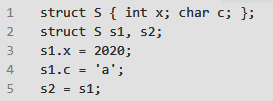
\includegraphics[width=0.5\textwidth]{picture2.2.png}
%  \caption{Primer kratkog segmenta koda}
%  \label{fig:slika2.2}
%\end{figure}

Pitanje na koje treba dati odgovor je kolika je struktura S, u bajtovima? Int je 4 bajta, a char jedan bajt, pa možda struktura S zauzima 5 bajtova? Pogrešno. Svi kompajleri za koje znamo zaokružiće veličinu struct S na ceo broj reči, u ovom slučaju 8 bajtova. Ukoliko to nije slučaj, kompajleri  se prisiljavaju da generišu zaista zastrašujući k\^od za pristup nizovima struct S-a na nekim arhitekturama. Dakle s1 zauzima 8 bajtova, ali će samo njih 5 biti inicijalizovano. Za zadatak s2 = s1, GCC generiše k\^od za kopiranje svih 8 bajtova u s2 bez obzira na njihovo značenje. Ako bi Memcheck jednostavno proveravao vrednosti redom kako su izašle iz memorije, “zaurlalo”  bi svaki put kad bi se desilo ovakvo dodeljivanje strukture. Dakle, neophodno je komplikovanije ponašanje opisano gore. Ovo omogućava GCC-u da kopira s1 u s2 na bilo koji način, a upozorenje će se emitovati samo ako se kasnije koriste neinicijalizovane vrednosti \cite{Memcheck}. 

\subsubsection{Bitovi važeće adrese (A bitovi)}
Prethodna sekcija opisuje kako se uspostavlja i održava valjanost vrednosti bez potrebe da se kaže da li program ima ili nema pravo na pristup bilo kojoj određenoj memorijskoj lokaciji. U ovoj sekciji ćemo razmotriti to pitanje.

Kao što je gore opisano, svaki bit u memoriji ili u procesoru ima pridruženi bit valjane vrednosti (V). Pored toga, svi bajtovi u memoriji, ali ne i u procesoru, imaju pridruženi bit valjane adrese (A, eng. \textit{valid-address bit}). Ovo ukazuje na to da li program može legitimno čitati ili pisati u tu lokaciju. To ne daje nikakve naznake valjanosti podataka na toj lokaciji, kako je to zadatak V bitova već samo da li se toj lokaciji može pristupiti ili ne. Svaki put kada vaš program čita ili upisuje u memoriju, \textit{Memcheck} proverava A bitove povezane sa adresom. Ako bilo koji od njih označi neispravnu adresu, prijavljuje se greška. Bitno je reći da sama čitanja i pisanja ne menjaju A bitove, već ih samo konsultuju.

Princip postavljanja, odnosno čišćenja A bitova je sledeći:
\begin{itemize}
\item Kada se program pokrene, sva globalna područja podataka su označena kao pristupačna.
\item Kada program izvrši \textit{malloc/new}, A bitovi za tačno dodeljeno područje, ni bajt više, označeni su kao dostupni. Po oslobađanju područja A bitovi se menjaju kako bi ukazali na nepristupačnost.
\item Kada se registar pokazivača steka (SP) pomeri gore ili dole, postavljaju se A bitovi. Pravilo je da je područje SP od vrha do podnožja steka označeni kao dostupno, a ispod SP nedostupno. 
%(Ako to zvuči nelogično, imajte na umu da stek raste prema dole, a ne prema gore, na gotovo svim Unix sistemima, uključujući GNU / Linux.) 
\item Pri obavljanju sistemskih poziva, A bitovi se odgovarajuće menjaju. Na primer, \textit{mmap} ''magično'' čini da se datoteke pojavljuju u adresnom prostoru procesa, pa se A bitovi moraju ažurirati ako \textit{mmap} uspe \cite{Memcheck}. 
\end{itemize}

Nakon svega navedenog dolazimo do rezimea \textit{Memcheck}-ovog principa funkcionisanja.
\begin{itemize}
\item[$\textendash$] Svaki bajt u memoriji ima 8 pridruženih V bitova (važeće vrednosti), govoreći da li bajt ima definisanu vrednost i jedan bit A (valjane adrese), odnosno govoreći da li program trenutno ima pravo da čita/piše na tu adresu. Kao što je gore pomenuto, velika upotreba kompresije znači da troškovi obično iznose oko 25\%.
\item[$\textendash$] Kada se memorija čita ili se u nju piše, pregledaju se odgovarajući A bitovi. Ako označe nevažeću adresu, \textit{Memcheck} emituje grešku neispravno čitanje (eng. \textit{invalid read}) ili neispravno pisanje (eng. \textit{invalid write}).
\item[$\textendash$] Kada se memorija čita u registre CPU-a, relevantni V bitovi se preuzimaju iz memorije i čuvaju u simuliranom CPU-u. Oni se ne konsultuju.
\item[$\textendash$] Kada se registar ispiše u memoriju, V bitovi za taj registar se takođe zapisuju nazad u memoriju.
\item[$\textendash$] Kada se vrednosti u registrima CPU koriste za generisanje memorijske adrese ili za određivanje ishoda uslovne grane, V bitovi za te vrednosti se proveravaju i emituje se greška ako je bilo koja od njih nedefinisana. Kada se vrednosti u registrima procesora koriste u bilo koju drugu svrhu, \textit{Memcheck} izračunava V bitove za rezultat, ali ih ne proverava.
\item[$\textendash$] Jednom kada se provere V bitovi za vrednost u CPU, oni se postavljaju da ukazuju na validnost. Ovo izbegava dugačke lance grešaka.
\item[$\textendash$] Kada se vrednosti učitaju iz memorije, \textit{Memcheck} proverava A bitove za tu lokaciju i izdaje upozorenje o nevalidnoj adresi ako je potrebno. U tom slučaju su učitani V bitovi primorani da označe validno stanje, uprkos tome što je lokacija nevalidna. Ovaj naizgled čudan izbor smanjuje količinu zbunjujućih informacija koje se predstavljaju korisniku. Izbegava neprijatnu pojavu u kojoj se memorija čita sa mesta koje je i nedostupno i sadrži nevažeće vrednosti, a kao rezultat toga dobićete ne samo grešku sa nevažećom adresom (čitanje / pisanje), već i potencijalno veliki skup greškaka neinicijalizovanih vrednosti - jedna za svaki put kada se vrednost koristi.
\end{itemize}

\textit{Memcheck} presreće pozive funkcija \textit{malloc, calloc, realloc, valloc, memalign, free, new, new[], delete i delete[]}. Ponašanje koje  se dobija usled toga je sledeće:
\begin{itemize}
\item \textit{malloc/new/new[]}: vraćena memorija je označena kao adresabilna, ali nema važeće vrednosti. To znači da u nju morate pisati pre nego što je pročitate.
\item \textit{calloc}: vraćena memorija označena je i adresabilnom i važećom, jer \textit{calloc} postavlja područje na nulu.
\item \textit{realloc}: ako je nova veličina veća od stare, novi odeljak je adresiran, ali nevažeći, kao kod \textit{malloc}-a. Ako je nova veličina manja, odloženi odeljak je označen kao nedostupan. \textit{Realloc}-u možete proslediti samo pokazivač koji vam je prethodno izdao \textit{malloc/calloc/realloc}.
\item \textit{free/delete/delete[]}: ovim funkcijama možete proslediti samo pokazivač koji vam je prethodno izdala odgovarajuća funkcija dodeljivanja. Inače, \textit{Memcheck} se žali. Ako je pokazivač zaista važeći, \textit{Memcheck} označava celo područje na koje pokazuje kao da ga nije moguće adresirati i postavlja blok u red oslobođenih blokova. Cilj je odložiti što je duže moguće realokaciju ovog bloka. Dok se to ne dogodi, svi pokušaji da mu se pristupi izazvaće grešku nevažeće adrese, kao što biste se nadali \cite{Memcheck}. 
\end{itemize}

\subsection{Greške nevalidnog čitanja/pisanja (eng. \textit{invalid read/write errors})}
\begin{figure}[!ht]
  \centering
  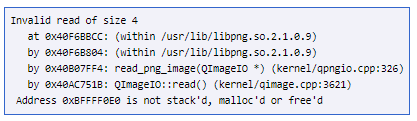
\includegraphics[width=0.7\textwidth]{invalidReadError.png}
  \caption{Primer ispisa greške nevalidnog čitanja, izvor: \cite{Memcheck}}
  \label{fig:slika2.3}
\end{figure}

Ove greške se javljaju kada vaš program čita ili piše u memoriju na mestu za koje \textit{Memcheck} smatra da ne bi trebalo. U ovom primeru, program je izvršio četvorobajtno čitanje na adresi 0xBFFFF0E0, negde unutar sistemske biblioteke \textit{libpng.so.2.1.0.9}, koja je pozvana negde drugde u istoj biblioteci, pozvana iz linije 326 \textit{qpngio.cpp} , i tako dalje.

\textit{Memcheck} će svakako pokušati da odredi na šta se ilegalna adresa može odnositi, jer je to često korisno. Dakle, ako pokazuje na blok memorije koji je već oslobođen, bićete obavešteni o tome, kao i o tome gde je blok oslobođen. Isto tako, ako se ispostavi da se nalazi na kraju hip bloka, što je greška, tj.~greška prekoračenja niza, bićete obavešteni o ovoj činjenici, kao i o tome gde je blok dodeljen. Ako koristite opciju \texttt{--read-var-info}, \textit{Memcheck} će raditi sporije, ali može dati detaljniji opis bilo koje nelegalne adrese.

U ovom primeru \textit{Memcheck} ne može da identifikuje adresu. Zapravo se adresa nalazi na steku, ali iz nekog razloga ovo nije važeća adresa steka - nalazi se ispod pokazivača steka i to nije dozvoljeno. U ovom konkretnom slučaju verovatno je uzrokovano GCC-om koji generiše nevažeći k\^od, što je poznata greška u nekim drevnim verzijama GCC-a.

Imajte na umu da vam \textit{Memcheck} samo govori da će vaš program uskoro pristupiti memoriji na nedozvoljenoj adresi i da pritom taj pristup ne može sprečiti. Dakle, ako vaš program pristupi, što bi obično rezultiralo greškom (segmentation fault), vaš program će i dalje imati isto ponašanje - ali od \textit{Memcheck}-a ćete dobiti poruku neposredno pre toga. U ovom konkretnom primeru čitanje ''smeća'' na steku nije fatalno, a program ostaje živ \cite{Memcheck}. 

\subsection{Korišćenje neinicijalizovanih vrednosti}
Greška pri korišćenju neinicijalizovane vrednosti se prijavljuje kada vaš program koristi vrednost koja nije inicijalizovana - drugim rečima, nije definisana. Ovde se nedefinisana vrednost koristi negde unutar printf mašine C biblioteke. Ova greška je prijavljena prilikom pokretanja programa sa listinga \ref{lst:slika2.4}, dok je njen ispis dat na slici \ref{fig:slika2.5}.

\begin{lstlisting}[caption={Program koji izaziva grešku korišćenja neinicijalizovanih vrednosti}, label={lst:slika2.4},language={C}] 
#include <stdio.h>
#include <stdlib.h>

int main(){
	int x;
	printf("%d\n", x);
	exit(EXIT_SUCCESS);
}
\end{lstlisting}

%\begin{figure}[!ht]
%  \centering
%  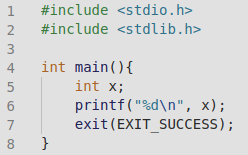
\includegraphics[width=0.5\textwidth]{uninitialisedErrorProgram.png}
%  \caption{Program koji izaziva grešku korišćenja neinicijalizovanih vrednosti}
%  \label{fig:slika2.4}
%\end{figure}

\begin{figure}[!ht]
  \centering
  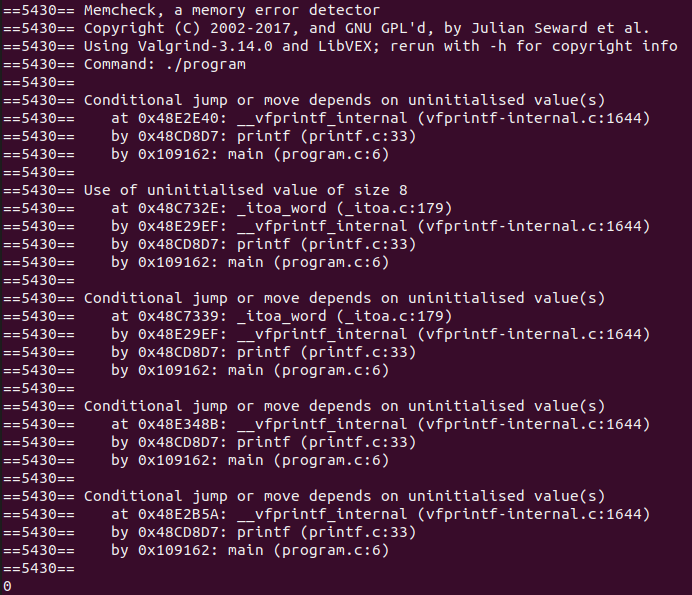
\includegraphics[width=0.7\textwidth]{uninitialisedError.png}
  \caption{Primer ispisa greške korišćenja neinicijalizovanih vrednosti}
  \label{fig:slika2.5}
\end{figure}

Važno je shvatiti da vaš program može kopirati neželjene (neinicijalizovane) podatke koliko god želi. \textit{Memcheck} to posmatra i evidentira podatke, ali se ne žali. Žalba se izdaje samo kada vaš program pokušava da koristi neinicijalizovane podatke na način koji može uticati na spolja vidljivo ponašanje vašeg programa. U ovom primeru, \textit{x} je neinicijalizovano. \textit{Memcheck} primećuje vrednost koja se prosleđuje \textit{\_IO\_printf} i odatle \textit{\_IO\_vfprintf}, ali ne daje komentar. Međutim, \textit{\_IO\_vfprintf} mora ispitati vrednost  kako bi je mogao pretvoriti u odgovarajući ASCI niz i \textit{Memcheck} se u ovom trenutku žali.

Izvori grešaka neinicijalizovanih vrednosti su sledeći:
\begin{itemize}
\item Lokalne promenljive u procedurama koje nisu inicijalizovane, kao u primeru iznad.
\item Sadržaj blokova hipa (dodeljen \textit{malloc}-om, \textit{new} ili sličnom funkcijom) pre nego što se nešto u tom bloku ispiše, odnosno pre inicijalizacije.
\end{itemize}

Da biste videli informacije o izvorima neinicijalizovanih podataka u svom programu, koristite opciju \texttt{--track-origins=yes}. Kao što je već rečeno, ovo čini \textit{Memcheck} sporijim, ali može znatno olakšati pronalaženje osnovnih uzroka neinicijalizovanih grešaka \cite{Memcheck}. 

\subsection{Korišćenje neinicializovane ili neadresirane vrednosti u sistemskom pozivu}

\textit{Memcheck} prati i proverava sve parametre sistemskih poziva. Svaki parametar se proverava pojedinačno, bio on inicijalizovan ili ne. Ukoliko sistemski poziv treba da čita iz bafera  koji je obezbeđen programu, \textit{Memcheck} proverava da li je ceo bafer adresiran i da li je njegov sadržaj inicijalizovan. Takođe, ako sistemski poziv treba da piše u bafer, \textit{Memcheck} proverava da li je bafer moguće adresirati. Nakon sistemskog poziva, \textit{Memcheck} ažurira sve parametre koje je pratio kako bi tačno odražavale sve promene u stanju memorije izazvane sistemskim pozivom.

\begin{lstlisting}[caption={Program koji izaziva grešku korišćenja neinicializovane ili neadresirane vrednosti u sistemskom pozivu, izvor: \cite{Memcheck}}, label={lst:slika2.6},language={C}] 
#include <unistd.h>
#include <stdlib.h>

int main(void){
	char* arr = malloc(10);
	int *arr2 = malloc(sizeof(int));
	write(1 /* stdout */, arr, 10);
	exit(arr2[0]);
}
\end{lstlisting}

%\begin{figure}[!ht]
%  \centering
%  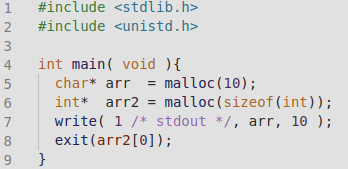
\includegraphics[width=0.5\textwidth]{sysCallErrorProgram.png}
%  \caption{Program koji izaziva grešku korišćenja neinicializovane ili neadresirane vrednosti u sistemskom pozivu, izvor: \cite{Memcheck}}
%  \label{fig:slika2.6}
%\end{figure}

\begin{figure}[!ht]
  \centering
  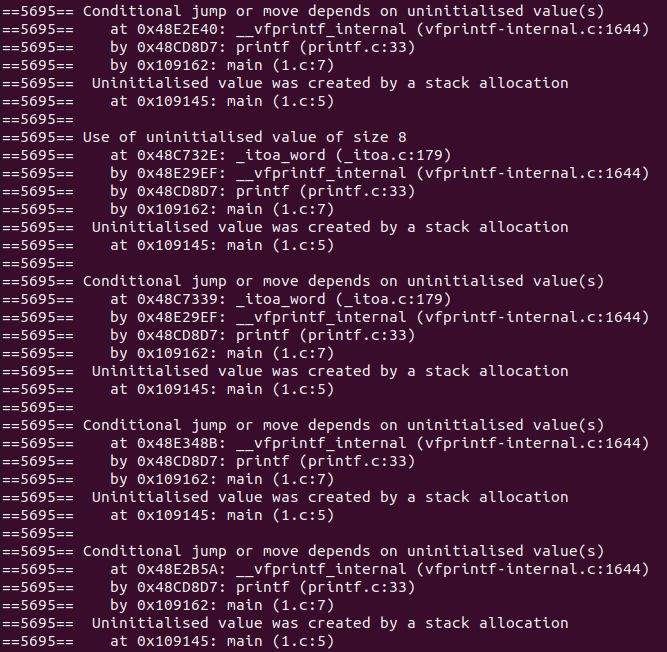
\includegraphics[width=0.7\textwidth]{sysCallError.png}
  \caption{Primer ispisa greške korišćenja neinicializovane ili neadresirane vrednosti u sistemskom pozivu}
  \label{fig:slika2.7}
\end{figure}

Na listingu \ref{lst:slika2.6} i slici \ref{fig:slika2.7} dat je primer programa koji ilustruje sistemski poziv sa neispravnim parametrima, kao i izveštaj koji dobijamo nakon analize pomenutog programa. Možemo da vidimo da je \textit{Memcheck} prikazao dve greške sa informacijama o korišćenju neinicijalizovanih vrednosti u sistemskim pozivima. Prva greška prikazuje da parametar \textit{arr} sistemskog poziva \textit{write()} pokazuje na neinicijalizovanu vrednost. Druga greška prikazuje da je podatak koji se prosleđuje sistemskom pozivu \textit{exit()} nedefinisan. Takođe, prikazane su i linije u samom programu gde se ove vrednosti koriste \cite{Memcheck}. 

\subsection{Nedopušteno oslobađanje memorije}
\textit{Memcheck} prati sve blokove memorije koje je program alocirao pomoću \textit{malloc/new}, tako da može tačno znati da li je argument prosleđen \textit{free/ delete} legitiman ili ne. Listing \ref{lst:slika2.8} ilustruje program koji je oslobodio isti blok dva puta. 

\begin{lstlisting}[caption={Program koji oslobađa isti blok dva puta}, label={lst:slika2.8},language={C}] 
#include <stdio.h>
#include <stdlib.h>

int main(){
	char *p;
	p = (char) malloc(5);
	p = (char) malloc(7);
	free(p);
	free(p);
	p = (char) malloc(9);
	exit(EXIT_SUCCESS);
}
\end{lstlisting}

%\begin{figure}[!ht]
%  \centering
%  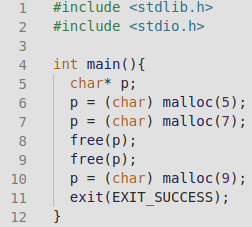
\includegraphics[width=0.5\textwidth]{invalidFreeErrorProgram.png}
%  \caption{Program koji oslobađa isti blok dva puta}
%  \label{fig:slika2.8}
%\end{figure}

Kao i kod grešaka nevalidnog čitanja/pisanja, \textit{Memcheck} pokušava da dokuči oslobođenu adresu. Ako je, kao ovde, slučaj da je adresa koja je prethodno oslobođena, to će biti prijavljeno i učiniće duplikate oslobađanja istog bloka lako uočljivim. Ovu poruku ćete dobiti i ako pokušate da oslobodite pokazivač koji ne pokazuje početak hip bloka. Slika \ref{fig:slika2.9} ilustruje izlaz dobijen puštanjem programa sa listinga \ref{lst:slika2.8} na analizu alatom \textit{Memcheck} \cite{Memcheck}. 

\begin{figure}[!ht]
  \centering
  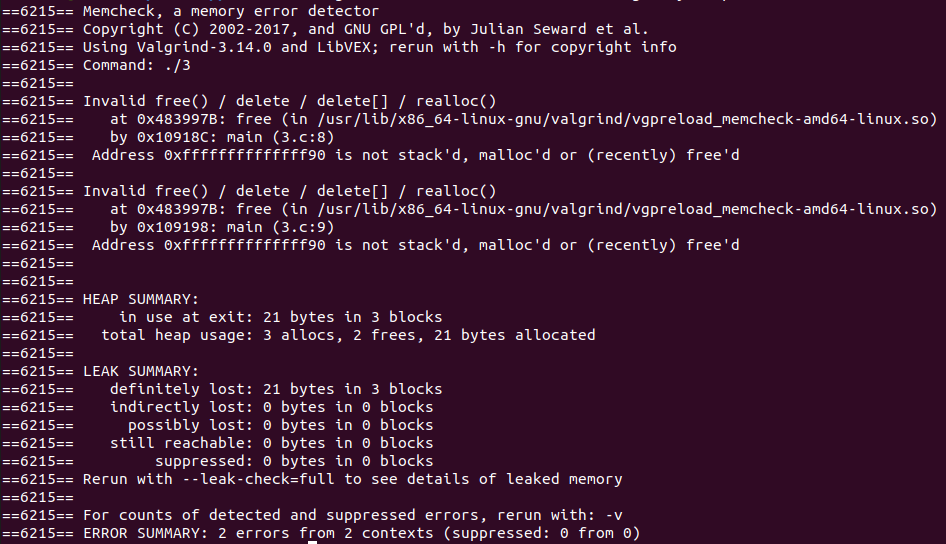
\includegraphics[width=0.7\textwidth]{invalidFreeError.png}
  \caption{Primer ispisa greške nedopuštenog oslobađanja memorije}
  \label{fig:slika2.9}
\end{figure}

\subsection{Preklapanje izvornog i odredišnog bloka}
Sledeće C bibliotečke funkcije kopiraju neke podatke iz jednog memorijskog bloka u drugi - \textit{memcpy, strcpy, strncpy, strcat, strncat}.  Blokovi na koje ukazuju njihovi pokazivači \textit{src} i \textit{dst} ne smeju se preklapati. \textit{POSIX} standardi imaju sledeću formulaciju: ''Ako se kopiranje vrši između objekata koji se preklapaju, ponašanje je nedefinisano''.  Stoga \textit{Memcheck} ovo proverava. Ukoliko dođe do preklapanja, prijaviće grešku.
\begin{figure}[!ht]
  \centering
  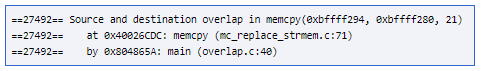
\includegraphics[width=0.7\textwidth]{overlapError.png}
  \caption{Primer ispisa greške preklapanja izvornog i odredišnog bloka, izvor: \cite{Memcheck}}
  \label{fig:slika2.10}
\end{figure}
Ne želite da se dva bloka preklapaju, jer bi jedan od njih mogao delimično da se prepiše kopiranjem. Može delovati da \textit{Memcheck} previše pedantno prijavljuje ovo u slučaju kada je \textit{dst} manji od \textit{src}. Na primer, očigledan način implementacije \textit{memcpy}  je kopiranje iz prvog bajta u poslednji. Međutim, vodiči za optimizaciju nekih arhitektura preporučuju kopiranje od poslednjeg bajta do prvog. Pouka priče je da ako zaista želite da napišete prenosivi k\^od, ne pravite nikakve pretpostavke o implentaciji jezika \cite{Memcheck}. 

\subsection{Sumnjive vrednosti argumenata}
Sve funkcije za alokaciju memorije uzimaju argument koji određuje veličinu memorijskog bloka koji treba dodeliti. Jasno je da tražena veličina treba da bude pozitivna vrednost koja obično nije preterano velika. Na primer, krajnje je neverovatno da veličina zahteva za dodelu premašuje ${2}^{63}$ bajta na 64-bitnoj mašini. Mnogo je verovatnije da je takva vrednost rezultat pogrešnog izračunavanja veličine i da je u stvari negativna vrednost (koja se čini preterano velikom jer se obrazac bita tumači kao nepotpisani celi broj). Takva vrednost se naziva ''sumnjivom vrednošću''. Argument veličine sledećih funkcija dodeljivanja biće proveren da li je sumnjiv: \textit{malloc, calloc, realloc, memalign, new, new[ ]. \_builtin\_new, \_builtin\_vec\_new}. Za \textit{calloc} se proveravaju oba argumenta.

Ukoliko dođe do ovakve sitruacije, prijaviće se greška sa slike \ref{fig:slika2.11} \cite{Memcheck}. 
\begin{figure}[!ht]
  \centering
  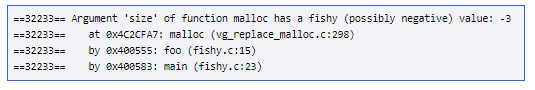
\includegraphics[width=0.7\textwidth]{fishyArgument.png}
  \caption{Primer ispisa greške sumnjive vrednosti argumenata, izvor: \cite{Memcheck}}
  \label{fig:slika2.11}
\end{figure}

\subsection{Detekcija curenja memorije}
\textit{Memcheck} evidentira podatke o svim blokovima hipa koji su alocirani tokom izvršavanja programa pozivom funkcija \textit{malloc/new} i dr.. Dakle, kada program prekine sa radom, \textit{Memcheck} zna koji blokovi nisu oslobođeni. Ukoliko je opcija \texttt{--leak-check}  adekvatno podešena, \textit{Memcheck} će za svaki neoslobođeni blok odrediti da li mu je moguće pristupiti preko pokazivača. 
Postoje dva načina da pristupimo sadržaju nekog memorijskog bloka preko pokazivača. Prvi način je preko pokazivača koji pokazuje na početak memorijskog bloka (eng. \textit{start-pointer}), dok je drugi način preko pokazivača koji pokazuje na sadržaj unutar memorijskog bloka (eng. \textit{interior-pointer}). Na nekoliko načina možemo saznati da li postoji pokazivač koji pokazuje na unutrašnjost nekog memorijskog bloka. Može se desiti da je postojao pokazivač koji je pokazivao na početak bloka, ali je namerno (ili nenamerno) pomeren da pokazuje na unutrašnjost bloka. Drugi slučaj jeste postojanje neželjene vrednosti u memoriji, koja je u potpunosti nepovezana i slučajna.

Imajući to na umu, na slici \ref{fig:slika2.12} navešćemo devet mogućih slučajeva kada pokazivači pokazuju na neke memorijske blokove.
\begin{figure}[!ht]
  \centering
  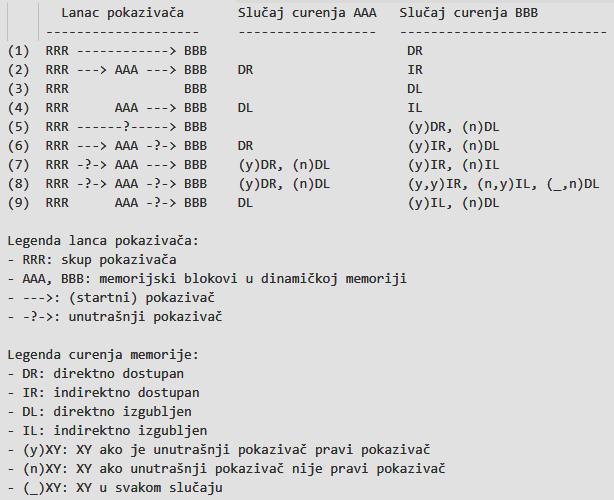
\includegraphics[width=0.7\textwidth]{memoryLeacking.png}
  \caption{Primer pokazivača na memorijski blok}
  \label{fig:slika2.12}
\end{figure}


Svaki mogući slučaj može se svesti na jedan od gore navedenih devet. \textit{Memcheck} objedinjuje neke od ovih slučajeva, što rezultira u sledeće četiri kategorije curenja memorije.
\begin{itemize}
\item[$\textendash$] \textbf{Još uvek dostupan (eng. \textit{still reachable})} – Ova klasa pokriva slučajeve 1 i 2 navedene na slici \ref{fig:slika2.12}. Pronađen je pokazivač na početak bloka ili više takvih pokazivača. Kako postoje pokazivači koji pokazuju na memorijsku lokaciju koja nije oslobođena, programer može da oslobodi memorijsku lokaciju neposredno pre završetka izvršavanja programa. Blokovi iz ove kategorije su vrlo česti i verovatno nisu problem. Dakle, \textit{Memcheck} podrazumevano neće pojedinačno prijavljivati takve blokove.
\item[$\textendash$] \textbf{Definitivno izgubljen (eng. \textit{definitely lost})} – Ova klasa pokriva slučaj 3 naveden na slici \ref{fig:slika2.12}. To znači da se ne može naći pokazivač na blok. Blok je klasifikovan kao ''izgubljen'', jer oslobađanje istog nije moguće na izlazu iz programa, kako na njega ne postoji pokazivač. Ovo je verovatno simptom gubitka pokazivača u nekom ranijem trenutku programa. Takve slučajeve treba da popravi programer.
\item[$\textendash$] \textbf{Indirektno izgubljen (eng. \textit{indirectly lost})} – Ova klasa pokriva slučajeve 4 i 9 navedene na slici \ref{fig:slika2.12}. To znači da je blok izgubljen, ne zato što na njega nema pokazivača, već zato što su svi blokovi koji na njega upućuju sami izgubljeni. Na primer, ako imate binarno stablo i koren se izgubi, svi njegovi čvorovi-potomci će se indirektno izgubiti. Budući da će problem nestati ako se popravi definitivno izgubljeni blok koji je prouzrokovao indirektno curenje, \textit{Memcheck} po default-u neće pojedinačno prijavljivati takve blokove sem ako nije podešena opcija \textit{–show-reachable=yes}.
\item[$\textendash$] \textbf{Moguće izgubljen (eng. \textit{possibly lost})} – Ova klasa obuhvata slučajeve 5-8 navedene na slici \ref{fig:slika2.12}. To znači da je pronađen jedan ili više pokazivača na memorijski blok, ali bar jedan od pokazivača je pokazuje na unutrašnjost memorijskog bloka. To bi mogla biti  slučajna vrednost u memoriji koja pokazuje na unutrašnjost bloka, što ne treba smatrati validnim sve dok se ne razreši slučaj pokazivača koji pokazuje na unutrašnjost bloka.
\end{itemize}

Treba napomenuti da ovo mapiranje devet mogućih slučajeva na četiri vrste curenja nije nužno najbolji način za prijavljivanje curenja. Naročito se prema unutrašnjim pokazivačima postupa nedosledno. Moguće je da će se kategorizacija u budućnosti poboljšati. Na slici  \ref{fig:slika2.13} dat je rezime curenja memorije koji ispisuje \textit{Memcheck}.
\begin{figure}[!ht]
  \centering
  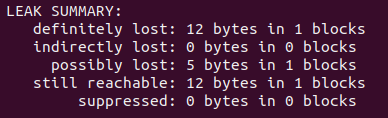
\includegraphics[width=0.7\textwidth]{leakResume.png}
  \caption{Rezime curenja memorije}
  \label{fig:slika2.13}
\end{figure}

Ako je uključena opcija \texttt{--leak-check = full}, \textit{Memcheck} će dati detaljan izveštaj za svaki definitivno izgubljeni ili moguće izgubljeni blok, uključujući i mesto gde je alociran. Međutim, \textit{Memcheck} vam ne može reći kada, kako ili zašto se izgubio pokazivač na iscureli blok, to morate sami da rešite. Generalno, treba težiti tome da vaši programi nemaju definitivno izgubljene ili moguće izgubljene blokove na izlazu.

Opcija \texttt{--show-leak-kind = <set>} kontroliše skup vrsta curenja koje će se prikazati kada je uključena opcija \texttt{--leak-check = full}. Inače, podrazumevana vrednost opcije \texttt{–leak-check} je \texttt{summary}.

\texttt{<set>} se definiše na jedan od sledećih načina:
\begin{enumerate}
\item Lista opcija odvojenih zarezom. Moguće opcije su: \texttt{definite, indirect, possible, reachable}.
\item \texttt{All} - za specifikaciju svih vrsta curenja.
\item \texttt{None} -  za prazan skup.
\end{enumerate}
Podrazumevana vrednost za vrste curenja koje se prikazuju je \texttt{--show-leak-kinds = definite, possible}.

Na slici \ref{fig:slika2.14} prikazan je izveštaj koji nam daje \textit{Memcheck} o definitivnom gubitku bloka veličine 12 bajta, još uvek dostupnom bloku veličine 12 bajta, moguće izgubljenom bloku veličine 5 bajta, kao i liniju u programu gde su oni alocirani. 
\begin{figure}[!ht]
  \centering
  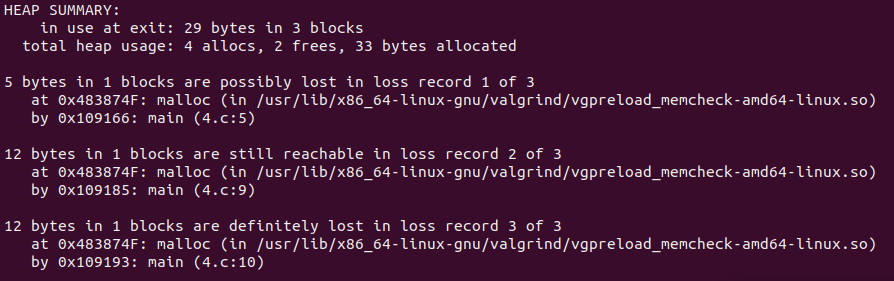
\includegraphics[width=0.7\textwidth]{heapResume.png}
  \caption{Izveštaj o curenju memorije}
  \label{fig:slika2.14}
\end{figure}

Budući da postoje različite vrste curenja memorije različitih težina, postavlja se pitanje koja curenja treba računati kao istinske ''greške'', a koja ne. \textit{Memcheck} koristi sledeći kriterijum:
\begin{itemize}
\item[$\textendash$] \textit{Memcheck} smatra da je curenje memorije ''greška'' samo ako je uključena opcija \texttt{--leak-check=full}. Drugim rečima, ako podaci o curenju memorije nisu prikazani, smatra se da to curenje nije ''greška''.
\item[$\textendash$] Definitivno i moguće izgubljeni blokovi se smatraju za pravu ''grešku'', dok indirektno izgubljeni i još uvek dospuni blokovi se ne smatraju kao greška \cite{Memcheck}. 
\end{itemize}

\section{Ostali važni alati Valgrind distribucije}

U ovoj sekciji biće obrađeni ostali važni alati \textit{Valgrind} distribucije. Biće reči o njihovoj osnovnoj nameni i načinu korišćenja. 

\subsection{Cachegrind}
Kako vremenom razlika između brzine RAM memorije i performansi koje obezbeđuje procesor eksponencijalno raste, merenje performansi keša postaje važna disciplina. Keš je zadužen da amortizuje tu razliku, a da bismo utvrdili koliko je on sposoban za to, prate se promašaji i pogodci u kešu. Jedna od  ideja za poboljšanje jeste da se smanji broj promašaja u kešu, prevashodno na nivou \textit{LL}.

\textit{Cachegrind} je alat koji simulira i prati pristup keš memoriji mašine na kojoj se program, koji se analizira, izvršava. Takođe, može se koristiti i za profajliranje izvršavanja grana. On simulira memoriju mašine, koja ima prvi nivo keš memorije podeljene u dve odvojene nezavisne sekcije: \textit{I1} - sekcija keš memorije u koju se smeštaju instrukcije i \textit{D1} - sekcija keš memorije u koju se smeštaju podaci, uz podršku objedinjenog drugog nivoa keša - \textit{L2}. Ovaj način konfiguracije odgovara mnogim modernim mašinama.


Međutim, neke moderne mašine imaju tri ili četiri nivoa keš memorije. Za ove mašine (u slučajevima kada \textit{Cachegrind} može automatski otkriti konfiguraciju keš memorije) \textit{Cachegrind} simulira pristup kešu prvog i poslednjeg nivoa, tj.~\textit{Cachegrind} simulira \textit{I1, D1 i LL}. Razlog za ovaj izbor je taj što keš memorija poslednjeg nivoa (\textit{LL}) ima najveći uticaj na vreme izvršavanja, jer maskira pristupe glavnoj memoriji. Dalje, \textit{L1} keš memorije često imaju malu asocijativnost, pa se njihovom simulacijom mogu otkriti slučajevi kada k\^od loše interaguje sa ovom keš memorijom.

\textit{Cachegrind} prikuplja sledeće statističke podatke o programu koji analizira:
\begin{itemize}
	\item Podaci o čitanjima instrukcija iz keš memorije uključuju sledeće statistike:\\
	\textit{Ir} - ukupan broj izvršenih instrukcija \\
	\textit{I1mr} - broj promašaja čitanja instrukcija iz keš memorije nivoa \textit{I1} \\
	\textit{ILmr} - broj promašaja čitanja instrukcija iz keš memorije nivoa \textit{LL}
	\item Podaci o čitanjima brze memorije uključuju sledeće statistike: \\
	\textit{Dr} - ukupan broj čitanja memorije \\
	\textit{D1mr} - broj promašaja čitanja nivoa keš memorije \textit{D1} \\ 
	\textit{DLmr} - broj promašaja čitanja nivoa keš memorije \textit{LL}
	\item Podaci o pisanjima u brzu memoriju uključuju sledeće statistike: \\
	\textit{Dw} - ukupan broj pisanja u memoriji \\
	\textit{D1mw} - broj promašaja pisanja u nivo keš memorije \textit{D1} \\
	\textit{DLmw} - broj promašaja pisanja u nivo keš memorije \textit{LL}
	\item Broj uslovno izvršenih grana - \textit{Bc} i broj promašaja uslovno izvršenih grana - \textit{Bcm}
	\item Broj indirektno izvršenih grana – \textit{Bi}  i broj promašaja indirektno izvršenih grana – \textit{Bim}.
\end{itemize}

Imajte na umu da ukupni pristup \textit{D1} jednak zbiru \textit{D1mr + D1mv}, a da je ukupni pristup \textit{LL} jednak zbiru \textit{ILmr + DLmr + DLmv}. Ova statistika se prikuplja na nivou celog programa, kao i pojedinačno na nivou funkcija. Postoji mogućnost da se dobije i broj pristupa skrivenoj memoriji za svaku liniju koda u originalnom programu. Na modernim mašinama \textit{L1} promašaj košta oko 10 procesorskih ciklusa, \textit{LL} promašaj košta oko 200 procesorskih ciklusa, a promašaji uslovno i inidirektno izvršene grane od 10 do 30 procesorskih ciklusa. Detaljno profajliranje keša i grana može biti vrlo korisno za razumevanje načina na koji vaš program komunicira sa mašinom, a samim tim i na taj način kako da to učinite bržim.

Što se rutine upotrebe \textit{Valgrind} alata tiče, uobičajeno je da kompajlirate program sa za debug mod (opcija \texttt{-g}). Međutim, za razliku od uobičajene upotrebe ostalih \textit{Valgrind} alata, sa \textit{Cachegrind}-om želimo još i uključenu optimizaciju, jer bi trebalo profajlirati program onako kako će se normalno izvršavati. 

Nakon kompilacije treba pokrenuti sam \textit{Cachegrind} da biste prikupili informacije o profajliranju, a zatim pokrenuti \texttt{cg\_annotate}, koji je u okviru paketa \textit{Valgrind}, da biste dobili detaljan prikaz tih informacija. Kao opcionalni međukorak, možete da koristite \texttt{cg\_merge} za sumiranje izlaza više pokretanja \textit{Cachegrind}-a u jednu datoteku koju zatim koristite kao ulaz za \texttt{cg\_annotate}. Alternativno, možete koristiti \texttt{cg\_diff} za razlikovanje više izlaza iz alata \textit{Cachegrind}, koje kasnije koristimo kao ulaz za \texttt{cg\_annotate}.

Da biste koristili alat \textit{Cachegrind} neophodno je podesiti opciju \texttt{–tool=cachegrind}. To ilustruje sledeća komanda. 
\begin{center}
\texttt{valgrind --tool=cachegrind [argumenti cachegrinda ] program [argumenti programa]}.
\end{center}

Izvršavanje programa trajaće veoma sporo, a po završetku štampaće se sažeti statistički podaci prikazani na slici \ref{fig:slika2.15}.
\begin{figure}[!ht]
  \centering
  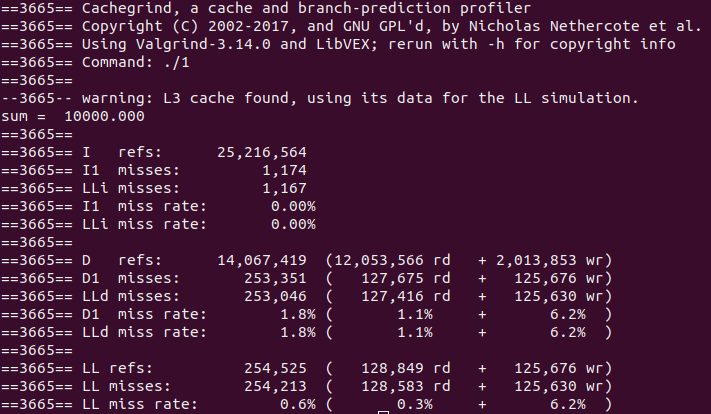
\includegraphics[width=0.7\textwidth]{CachegrindReport.png}
  \caption{Izveštaj alata \textit{Cachegrind}}
  \label{fig:slika2.15}
\end{figure}
Statistika predviđanja grana se ne prikuplja po default-u. Da biste to omogućili, dodajte opciju \texttt{--branch-sim = yes}.

Pored štampanja rezimea na standardni izlaz, \textit{Cachegrind} u datoteku upisuje i detaljnije informacije o profajliranju. Podrazumevano se ova datoteka naziva \texttt{cachegrind.out.<pid>} (gde je <pid> ID procesa koji se izvršio), ali njeno ime se može promeniti pomoću opcije \texttt{--cachegrind-out-file}. Ova datoteka je čitljiva za ljude, ali je pre svega namenjena tumačenju pratećeg programa \texttt{cg\_annotate}.

Da biste dobili rezime funkciju po funkciju, pokrenite komandu
\begin{center}
\texttt{cg\_annotate <filename>},
\end{center}
gde je <filename> \textit{Cachegrind} izlazna datoteka.

Prvi deo izveštaja prikazan je na slici \ref{fig:slika2.16}. On obuhvata informacije o konfiguraciji keša (\textit{I1, D1, LL}), komandu pokretanja programa koji se ispituje, koji su događaji praćeni itd.. 
\begin{figure}[!ht]
  \centering
  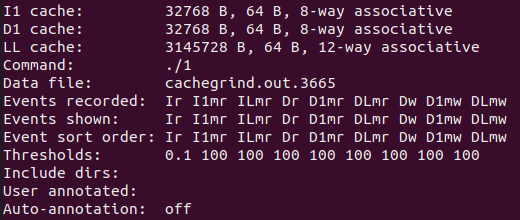
\includegraphics[width=0.7\textwidth]{CgAnotateFirst.png}
  \caption{Prvi deo izveštaja dobijenog primenom cg\_anotate}
  \label{fig:slika2.16}
\end{figure}

Nakon toga sledi izveštaj na nivou celog programa prikazan na slici \ref{fig:slika2.17}. On je sličan rezimeu datom kada \textit{Cachegrind} završi sa radom uz dodatu statistiku fukcija po funkcija. Svaka funkcija je identifikovana parom \textit{ime\_datoteke: ime\_funkcije}. Ako kolona sadrži samo tačku, to znači da funkcija nikada ne izvodi taj događaj. Ime \textit{???} koristi se ako se ime datoteke i/ili ime funkcije ne može utvrditi iz informacija o otklanjanju grešaka. Ako većina unosa ima oblik \textit{???: ???} program verovatno nije kompajliran sa opcijom \texttt{-g} \cite{Cachegrind}. 
\begin{figure}[!ht]
  \centering
  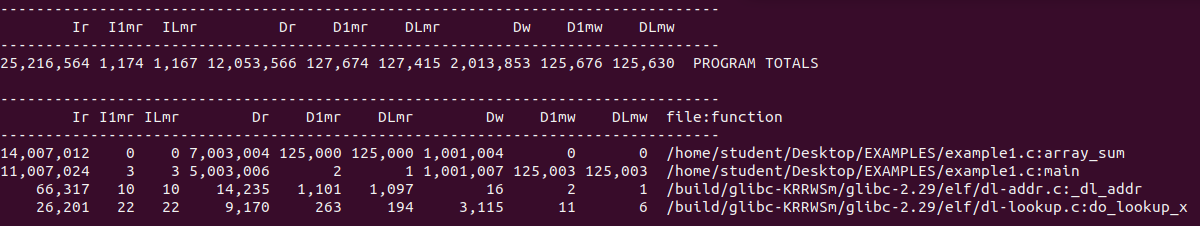
\includegraphics[width=0.7\textwidth]{CgAnotateSecond.png}
  \caption{Drugi deo izveštaja dobijenog primenom cg\_anotate}
  \label{fig:slika2.17}
\end{figure}

\subsection{Callgrind}
\textit{Callgrind} je alat za profajliranje koji generiše istoriju poziva funkcija korisničkog programa u vidu grafa. Bazično, sakupljeni podaci sastoje se od broja izvršenih instrukcija, njihov odnos sa linijama izvršnog koda, odnos pozivaoc/pozvan između funkcija, kao i broj takvih poziva. Opciono, simulacija keš memorije i/ili profajliranje grana (slično \textit{Cachegrind}-u) mogu dati dodatne informacije o ponašanju aplikacije u toku izvršavanja. 

Podaci dobijeni profajliranjem ispisuju se u datoteku po završetku rada alata i programa. Za prezentaciju podataka i interaktivnu kontrolu profajliranja obezbeđena su dva alata komandne linije.
\begin{itemize}
\item \textbf{callgrind\_annotate} - Ovaj alat čita generisani fajl i ispisuje sortirane liste funkcija, opciono sa anotacijom izvora. Za grafičku vizuelizaciju podataka, preporučuju se dodatni alat \textit{KCachegrind}, GUI zasnovan na KDE / Qt, koji olakšava navigaciju velikom količinom podataka koje proizvodi \textit{Callgrind}.
\item \textbf{callgrind\_control} - Ovaj alat vam omogućava da interaktivno posmatrate i kontrolišete status programa koji se trenutno izvodi pod kontrolom \textit{Callgrind}-a, bez zaustavljanja programa. Možete dobiti statističke podatke kao npr. stanje steka, a u svakom trenutku se takođe može generisati i profil.
\end{itemize}

Alat \textit{Cachegrind} sakuplja podatke, odnosno broji događaje koji se dešavaju direktno u jednoj funkciji. Ovaj mehanizam sakupljanja podataka se naziva ekskluzivnim. Alat \textit{Callgrind} proširuje ovu funkcionalnost tako što propagira cenu funkcije preko njenih granica. Na primer, ako funkcija \textit{foo} poziva funkciju \textit{bar}, cena funkcije \textit{bar} se dodaje funkciji \textit{foo}. Kada se ovaj mehanizam primeni na celu funkciju, dobija se slika takozvanih inkluzivnih poziva, gde cena svake funkcije uključuje i cene svih funkcija koje ona poziva, direktno ili indirektno.

Zahvaljujući grafu poziva, može da se odredi, počevši od main funkcije, koja funkcija ima najveću cenu poziva. Pozivaoc/pozvan cena je izuzetno korisna za profajliranje funkcija koje imaju više poziva iz raznih funkcija, i gde imamo priliku za optimizaciju našeg programa menjajući k\^od u funkciji koja je pozivaoc, tačnije redukovanjem broja poziva. Važno je napomenuti da mogućnost detektovanja svih poziva funkcija, kao i zavisnost instrukcija alata \textit{Callgrind} zavisi od platforme na kojoj se izvršava. Ovaj alat najbolje radi na \textit{x86 i amd64}, ali nažalost ne daje najtačnije rezultate na platformama \textit{PowerPc, ARM i MIPS}. Razlog je taj što kod navedenih platformi ne postoji eksplicitan poziv ili instrukcija u skupu instrukcija, pa \textit{Callgrind} mora da se oslanja na heuristike da bi detektovao pozive ili instrukcije.

Kao i kod \textit{Cachegrind}-a, da bi uspešno analizirali program koristeći \textit{Callgrind}, program kompajliramo za debug mod (opcija \texttt{-g}) i sa uključenom optimizacijom. Da biste koristili ovaj alat, morate navesti \texttt{--tool = callgrind} u komandnoj liniji \textit{Valgrind}-a. To ilustruje sledeća komanda.
\begin{center}
\texttt{valgrind --tool=callgrind [opcije callgrinda] program [argumenti programa]}.
\end{center}

Nakon završetka programa i rada alata, generiše se datoteka podataka profila koja se zove \texttt{callgrind.out.<pid>}, gde je <pid> ID procesa programa koji se profajlira. Da biste generisali rezime funkciju po funkciju koristeći pomenutu datuteku, iskoristite sledeću komandu:
\begin{center}
\texttt{callgrind\_annotate [dodatni argumenti] callgrind.out.<pid>}.
\end{center}

Ovaj rezime je sličan izlazu koji dobijete  pokretanjem \textit{Cachegrind}-a sa \texttt{cg\_annotate} -  lista funkcija je poređana po ekskluzivnim troškovima funkcija, koje su takođe  prikazane \cite{Callgrind}. 

Na slici \ref{fig:slika2.18} prikazana vizuelizacija izveštaja \textit{Callgrind}-a korišćenjem alata \textit{KCashegrind}.
\begin{figure}[!ht]
  \centering
  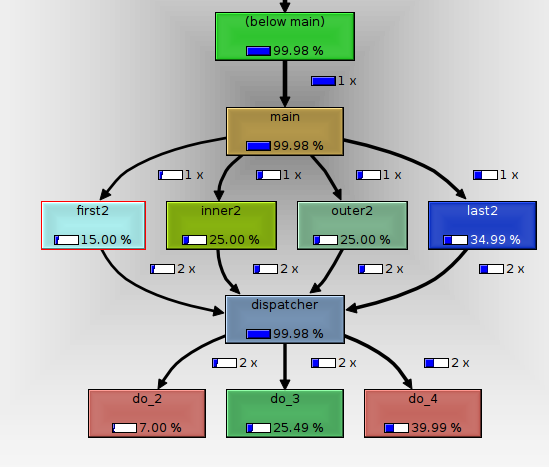
\includegraphics[width=0.7\textwidth]{MUjHe.png}
  \caption{Primer vizuelizacije izveštaja, izvor: Stack Overflow}
  \label{fig:slika2.18}
\end{figure}

\subsection{Helgrind}\label{HelgrindSection}
\textit{Helgrind} je \textit{Valgrind}-ov alat za otkrivanje grešaka sinhronizacije u programima C, C++ i Fortran prilikom upotreba modela niti \textit{POSIX}. Glavne apstrakcije modela niti  \textit{POSIX} su: skup niti koji dele zajednički adresni prostor, formiranje niti, spajanje niti, izlaz iz funkcije niti, muteksi (katanci), uslovne promenljive (obaveštenja o događajima među nitima), čitaj-piši zaključavanje, spinlokovi, semafori i barijere.

\textit{Helgrind} može otkriti sledeća tri tipa grešaka:
\begin{enumerate}
	\item Pogrešna upotreba \textit{POSIX} API-ja
	\item Potencijalno blokiranje prouzrokovano redosledom zaključavanja
	\item Trka sa podacima - pristup memoriji bez odgovarajućeg zaključavanja ili sinhronizacije
\end{enumerate}

Problemi poput ovih često rezultiraju ponovljivim padovima, vremenski zavisnim padovima, mrtvim tačkama i drugim nepravilnim ponašanjem, a koji se teško mogu pronaći drugim sredstvima.

\textit{Helgrind} najbolje funkcioniše kada vaša aplikacija koristi samo interfejs za rad sa nitima \textit{POSIX}. Međutim, ako želite da koristite korisnički prilagođene niti, možete opisati njihovo ponašanje \textit{Helgrind}-u koristeći makro \texttt{ANNOTATE\_*} definisan u \textit{helgrind.h}.

Da biste koristili ovaj alat, morate navesti \texttt{--tool = helgrind} u komandnoj liniji \textit{Valgrind}-a.

\subsubsection{Pogrešna upotreba POSIX API-ja}
\textit{Helgrind} presreće pozive ka funkcijama biblioteke \textit{pthread}, i zbog toga je u mogućnosti da otkrije veliki broj grešaka. Za sve \textit{pthread} funkcije koje \textit{Helgrind} presreće generiše se podatak o grešci ako funkcija vrati k\^od greške, i ako \textit{Helgrind} nije našao greške u kodu. Ovakve greške mogu da dovedu do nedefinisanog ponašanja programa i do pojave grešaka u programima koje je kasnije veoma teško otkriti.

Greške koje mogu biti otkrivene su:
\begin{itemize}
\item Greške u otključavanju muteksa – slučaj nevažećeg muteksa, nezaključanog muteksa, ili muteksa zaključanog od strane druge niti.
\item Greške u radu sa zaključanim muteksom – uništavanje nevažećeg ili zaključanog muteksa, rekurzivno zaključavanje nerekurzivnog muteksa, oslobađanje memorije koja sadrži zaključan muteks.
\item Prosleđivanje muteksa kao argumenta funkcije koja očekuje kao argument reader-writer lock i obrnuto.
\item Greške sa \textit{pthread barrier} - nevažeća ili dupla inicijalizacija, uništavanje \textit{pthread barrier} koji nikada nije inicijalizovan ili koga niti čekaju ili čekanje na objekat koji nije nikada inicijalizovan.
\item Greške prilikom korišćenja funkcije \textit{pthread\_cond\_wait} - prosleđivanje nezaključanog, nevažećeg ili muteksa koga je zaključala druga nit.
\item \textit{Pthread} funkcija vrati k\^od greške koji je potreno dodatno obraditi, kada se nit uništi, a da još drži zaključanu promeljivu.
\item Nekonzistentne veze između uslovnih promeljivih i njihovih odgovarajućih muteksa.
\end{itemize}

Provere koje se odnose na mutekse se takođe primenjuju i na reader-writer lock. Prijavljena greška prikazuje i primarno stanje steka koje pokazuje gde je detektovana greška. Takođe, ukoliko je moguće ispisuje se i broj linije u izvornom  kodu gde se greška nalazi. Ukoliko se greška odnosi na muteks, \textit{Helgrind} će prikazati i gde je prvi put detektovao problematični muteks.

%\begin{figure}[!ht]
%  \centering
%  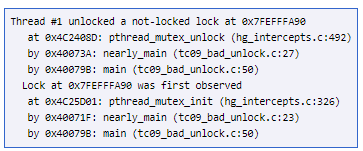
\includegraphics[width=0.7\textwidth]{HelgrindFirst.png}
%  \caption{Primer prikaza greške u programu, izvor: \cite{Helgrind}}
%  \label{fig:komenatar1}
%\end{figure}

\subsubsection{Potencijalno blokiranje niti}
\textit{Helgrind} nadgleda redosled kojim niti zaključavaju promenljive. To mu omogućava detektovanje potencijalnih zastoja koji bi mogli nastati formiranjem ciklusa zaključavanja. Na ovaj način je moguće detektovati greške koje se nisu javile tokom samog procesa testiranja programa, već se javljaju kasnije tokom korišćenja istog.

Šta tačno predstavlja ovakav tip greške, ilustrovaćemo primerom:\\
Zamislimo da imamo zajednički resurs R, kome da bi pristupili moramo da zaključamo dve promenljive L1 i L2. Pretpostavimo zatim da dve niti N1 i N2 žele da pristupe deljenoj promenljivoj R. Do blokoranja niti dolazi kada nit N1 zaključa L1, a u istom trenutku N2 zaključa L2. Nakon toga nit N1 ostane blokirana jer čeka da se otključa L2, ne bi li je zaključao, a analogno tome nit N2 ostane blokirana jer čeka da se otključa L1.

\textit{Helgrind} kreira usmereni graf koji predstavlja sve promenljive koje se mogu zaključati, a koje je otkrio u prošlosti. Kada nit naiđe na novu promenljivu koju zaključava, graf se ažurira i proverava se da li graf sadrži ciklus u kome se nalaze zaključane promenljive. Postojanje kruga u kome se nalaze zaključane promenljive je signal da je moguće da će doći do blokiranja niti tokom izvršavanja.

Generalno, \textit{Helgrind} će odabrati dve zaključane promenljive uključene u ciklus i pokazati vam kako je narušena konzistentnost. To čini tako što prikazuje programske tačke koje su prvo definisale redosled i programske tačke koje su ga kasnije prekršile. Ako postoje više od dve zaključane promenljive u krugu problem je još ozbiljniji.

%\begin{figure}[!ht]
%  \centering
%  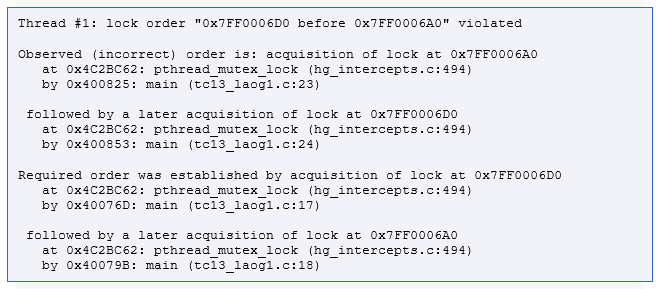
\includegraphics[width=0.7\textwidth]{HelgrindTwo.png}
%  \caption{Primer prikaza greške u programu, izvor: \cite{Helgrind}}
%  \label{fig:komentar2}
%\end{figure}

\subsubsection{Trka sa podacima}
Trka sa podacima (eng. \textit{data races}) nastaje, odnosno može nastati usled korišćenja deljene memorije bez adekvatnog zaključavanja ili sinhronizacije, a u cilju omogućavanja pristupa samo jednoj niti. Obezbeđivanje programa bez trke sa podacima je jedna od centralnih poteškoća programiranja sa nitima. 

Primer sa slike \ref{fig:slika2.20} ilustruje program u kom se koristi promenljiva bez adekvatne sinhronizacije.
\begin{figure}[!ht]
  \centering
  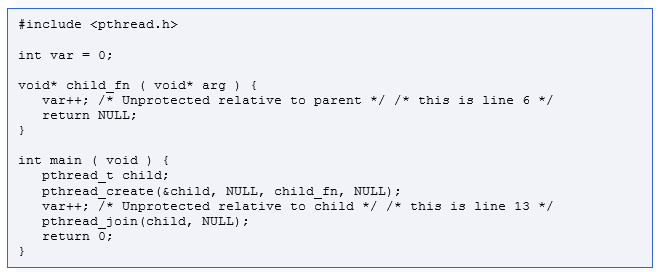
\includegraphics[width=0.8\textwidth]{DataRace.png}
  \caption{Primer programa koji koristi promenljivu sa neadekvatnom sinhronizacijom, izvor: \cite{Helgrind}}
  \label{fig:slika2.20}
\end{figure}

U ovom programu je nemoguće znati kolika je vrednost \textit{var} na kraju rada programa. Da li je 2 ili 1? Razlog tome je što ništa ne sprečava da obe niti (roditelj i dete) da pristupe i promene vrednost promenljive \textit{var}. Ispravan program bi zaštitio \textit{var} katancem tipa \textit{pthread\_mutex\_t}, koja se dobija pre svakog pristupa i oslobađa nakon toga. Izlaz \textit{Helgrind}-a za program sa slike \ref{fig:slika2.20} prikazan je na slici \ref{fig:slika2.21}:
\begin{figure}[!ht]
  \centering
  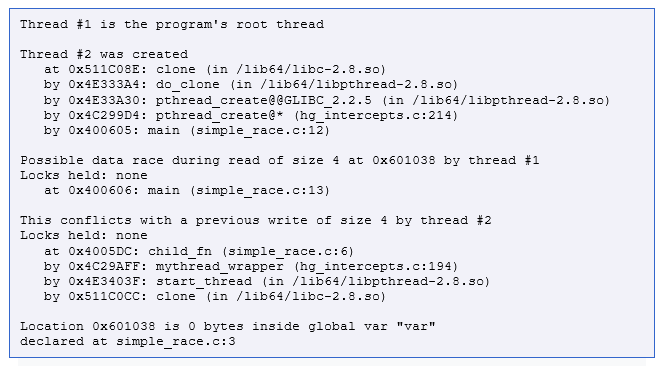
\includegraphics[width=0.8\textwidth]{DataRaceReport.png}
  \caption{Izveštaj \textit{Helgrind}-a za korišćenje promenljive bez adekvatne sinhronizacije, izvor: \cite{Helgrind}}
  \label{fig:slika2.21}
\end{figure}

U izveštaju koji je prikazan na slici \ref{fig:slika2.21} možemo tačno da vidimo koje niti pristupaju promenljivoj bez sinhronizacije, gde se vrši sam pristup promenljivoj, ime i veličinu same promenljive kojoj niti pristupaju. Prikazivanje osnovnih informacija promenljivih nema dodatnih troškova tokom izvršavanja, nakon što se \textit{Helgrind} pokrene i pokrene vaš program. Međutim, \textit{Helgrind} će potrošiti znatno više vremena i memorije prilikom pokretanja programa kada je aktivna opcija čitanja informacija za debagovanje. Stoga je ova opcija podrazumevano onemogućena. Da biste je omogućili, trebate \textit{Helgrind}-u dati opciju \texttt{--read-var-info = yes}.

Algoritam za detekciju pristupa promenljivoj bez sinhronizacije baziran je na ''desilo se pre'' relaciji (eng. \textit{happens-before relation}). Kada kažemo da su dva pristupa promenljivoj od strane dve različite niti u ''relaciji desilo se pre'', to znači da postoji neki lanac operacija sinhronizacije među nitima zbog kojih se ti pristupi dešavaju u određenom redosledu, bez obzira na stvarne brzine napretka pojedinačnih niti. Ovo je neophodno svojstvo da bi program koji radi sa nitima bio pouzdan, zbog čega ga \textit{Helgrind} proverava. \textit{Helgrind} presreće precizno definisan skup događaja na kojima počiva relacija ''desilo se pre'' i kreira usmereni aciklični graf koji predstavlja sve ''desilo se pre'' relacije u programu. Pored toga, on prati i sve pristupe memoriji u programu. Ako promenljivoj pristupaju dve različite niti, ali \textit{Helgrind} ne može da pronađe nijednu putanju od prvog pristupa do drugog kroz promenuti graf, onda izveštava grešku o trci sa podacima \cite{Helgrind}.  

\subsection{DRD}
\textit{DRD} je \textit{Valgrind}-ov alat za otkrivanje grešaka u višenitnim programima C i C++. Alat radi za bilo koji program koji koristi niti bazirane na modelu \textit{POSIX}.

U zavisnosti od toga koja se višenitna paradigma koristi u programu, može se pojaviti jedna ili više sledećih grešaka:
\begin{itemize}
\item Trka sa podacima;
\item Zadržavanje katanaca - jedna nit blokira napredovanje jedne ili više drugih niti držeći predugo katanac zaključanim;
\item Pogrešna upotreba \textit{POSIX} API-ja;
\item Potencijalno blokiranje prouzrokovano redosledom zaključavanja;
\item Lažno deljenje - ako niti koje rade na različitim procesorskim jezgrima često pristupaju različitim promenljivim smeštenim u istoj liniji keš memorije, to će usporiti uključene niti zbog česte razmene linija keš memorije.
\end{itemize} 

\textit{DRD} i \textit{Helgrind} ne koriste iste algoritme za otkrivanje grešaka, pa samim tim ne otkrivaju iste tipove grešaka.
Što se tiče grešaka vezanih za pogrešnu upotrebu \textit{POSIX} API-ja, kao i trke sa podacima, greške koje \textit{DRD} otkriva su identične onim koje otkriva \textit{Helgrind}, a koje su opisane u sekciji \ref{HelgrindSection},  uz određene minimalne razlike.

Kada je u pitanju greška vezana za trku sa podacima, \textit{DRD} ispisuje poruku svaki put kada otkrije da je došlo do trke podataka. Svakako treba imati na umu sledeće činjenice prilikom tumačenja izlaza \textit{DRD}-a. Alat \textit{DRD} svakoj niti dodeljije jedinstveni ID broj. Brojevi koji se dodeljuju nitima u svojstvu identifikatora počinju od jedinice i dodeljuju se jednokratno. Termin segment se odnosi na uzastopni niz  operacija učitavanja, skladištenja i sinhronizacije - sve izvršene u istoj niti. Segment uvek započinje i završava se operacijom sinhronizacije. Analiza trke sa podacima vrši se između segmenata, a ne između pojedinačnih operacija učitavanja i skladištenja iz razloga boljih performansi. Uvek postoje najmanje dva pristupa memoriji uključena u trku podataka. Pristupi memoriji uključeni u trku podataka nazivaju se sukobljenim pristupima memoriji. \textit{DRD} štampa izveštaj za svaki pristup memoriji koji je u sukobu sa prethodnim pristupom memoriji. Na slici \ref{fig:slika2.22} dat je izlaz iz alata \textit{DRD} nakon što je došlo do trke sa podacima u programu. 
\begin{figure}[!ht]
  \centering
  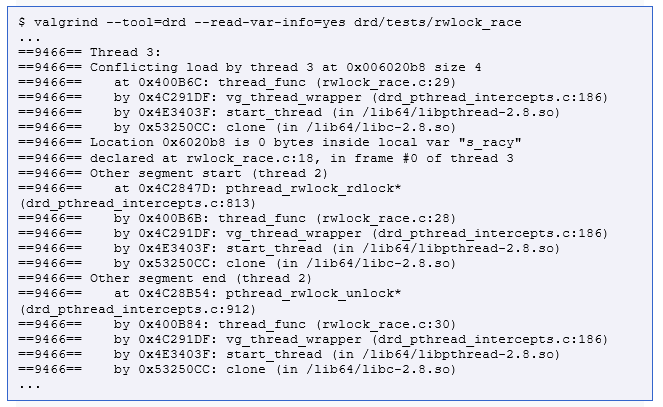
\includegraphics[width=0.8\textwidth]{DRDDataRaceReport.png}
  \caption{Izveštaj \textit{DRD}-a o trci sa podacima, izvor: \cite{Drd}}
  \label{fig:slika2.22}
\end{figure}

Niti moraju biti u stanju da napreduju, a da ih druge niti predugo ne blokiraju. Ponekad nit mora da sačeka dok muteks ili objekat sinhronizacije reader-writer ne otključa druga nit. Pojava u kojoj jedna nit ne može da nastavi sa radom zbog blokiranja drugih niti naziva se zadržavanje katanaca  (eng. \textit{lock contention}). Ovakva pojava je nepoželjna u višenitnim sistemima, a u njenom otklanjanju pomaže alat \textit{DRD} koji otkriva ovaj tip problema. Zadržavanje katanaca uzrokuje kašnjenja. Takva kašnjenja treba da budu što kraća. Dve opcije komandne linije \texttt{--exclusive-threshold=<n> i --shared-threshold=<n>} omogućavaju otkrivanje prekomernog zadržavanja katanaca tako što \textit{DRD} prijavljuje svako zaključavanje koje je zadržano duže od navedenog praga \cite{Drd}. 

Da biste koristili ovaj alat, morate navesti \texttt{--tool = drd} u komandnoj liniji \textit{Valgrind-a.}

\subsection{Massif}
\textit{Massif} je alat za analizu hip memorije korisničkog programa. Meri koliko memorije hipa vaš program koristi i na koji način. To obuhvata memoriju kojoj korisnik može pristupiti, kao i memoriju koja se koristi za dodatne koncepte poput book-keeping bajtova i prostora za poravnanje. Takođe, može izračunati i veličinu stek memorije vašeg programa, s tim da ova opcija nije podrazumevana, već se mora eksplicitno navesti.

Profajliranje hipa vam može pomoći da smanjite količinu memorije koju vaš program koristi. Na modernim mašinama sa virtuelnom memorijom to će doprineti određenim pogodnostima. To može ubrzati vaš program, kako manji programi imaju bolju iskorišćenost keša i izbegavaju straničenje. S druge strane, ako vaš program zahteva puno memorije, dobra iskorišćenost hipa će smanjiti šansu za izgladnjivanjem prostora za razmenu (eng. \textit{swap space}) korisničke mašine. 

Postoje određeni tipovi curenja memorije koji ne mogu biti otkriveni klasičnim alatima koji vrše analizu curenja memorije, poput \textit{Memcheck}-a. To je zato što memorija zapravo nikada nije izgubljena, pokazivač na nju i dalje postoji, ali nije u upotrebi. Programi koji imaju ovakvo curenje mogu s vremenom nepotrebno povećati količinu memorije koju koriste. \textit{Massif} može pomoći u identifikovanju ovakvog tipa curenja memorije.

Važno je znati da vam \textit{Massif} ne daje samo informaciju koliko hip memorije koristi vaš program, već takođe daje vrlo detaljne informacije koje ukazuju na to koji su delovi vašeg programa odgovorni za alociranje te memorije.

Pre svega, kao i za ostale \textit{Valgrind} alate, trebalo bi kompajlirati program za debag mod (opcija \texttt{-g}). U ovom slučaju nije presudno važno sa kojim nivoom optimizacije kompajlirate program, jer je malo verovatno da će to uticati na upotrebu memorije hipa.

Nakon kompilacije željenog programa treba pokrenuti sam \textit{Massif} da biste prikupili informacije o profajliranju, nakon čega treba pokrenuti \texttt{ms\_print} da biste ih predstavili na čitljiv način. Da biste koristili ovaj alat, morate navesti \texttt{--tool = massif} u komandnoj liniji \textit{Valgrind}-a.
\begin{center}
\texttt{valgrind --tool=massif [argumenti massifa] program [argumenti programa]}
\end{center}
 
Program koji se izvršava pod alatom \textit{Massif} će raditi veoma sporo. Po završetku rada programa i alata, svi podaci o profajliranju zapisuju se u datoteku. Podrazumevano se ova datoteka naziva \texttt{massif.out.<pid>}, gde je <pid> ID procesa, iako se ovo ime datoteke može promeniti pomoću opcije \texttt{--massif-out-file}. Kao što je već rečeno, da bi informacije koje je \textit{Massif} sakupio mogli da vidimo u čitljivom formatu, koristimo \texttt{ms\_print} nad izlaznom datotekom alata \textit{Massif}, npr. \texttt{massif.out.12345}.

\begin{center}
\texttt{ms\_print massif.out.12345}
\end{center}

\texttt{ms\_print} prozvodi graf koji prikazuje potrošenju memorije tokom izvršavanja programa, kao i detaljne informacije o različitim tačkama programa koje su odgovorne za alokaciju memorije. Korišćenje različitih skripti za prezentaciju rezultata je namerno, u cilju odvajanja sakupljanja podataka od prezentacije, što znači da je moguće dodati nov način prikaza podataka u svakom trenutku. Na slici \ref{fig:slika2.23} vidimo izlaz iz alata \textit{Massif} prikazan pomoću \texttt{ms\_print}.
\begin{figure}[!ht]
  \centering
  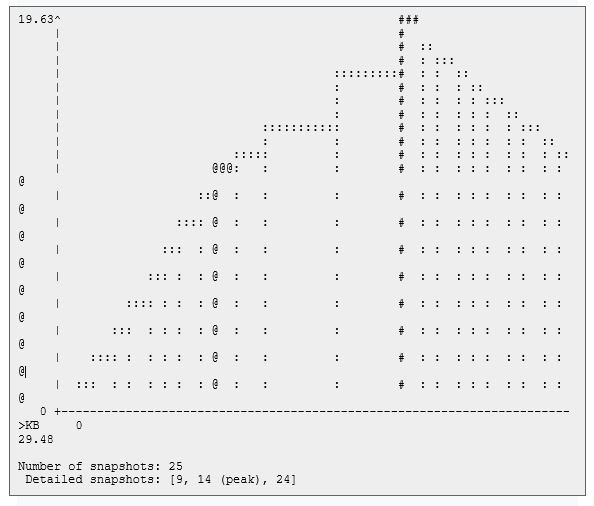
\includegraphics[width=0.7\textwidth]{MassifPhoto.png}
  \caption{Primer opterećenja hipa korišćenjem alata \textit{Massif}, izvor: \cite{Massif}}
  \label{fig:slika2.23}
\end{figure}

Važno je naglasiti da alat \textit{Massif} meri samo hip memoriju, odnosno memoriju koja je alocirana koristeći \textit{malloc, calloc, realloc, memalign, new, new[]} i nekoliko drugih sličnih funkcija. Ovo znači da \textit{Massif} ne meri memoriju koja je alocirana sistemskim pozivima nižeg nivoa kao što su \textit{mmap, mremap i brk}. Iako  u programu mogu postojati sistemski pozivi za alociranje memorije, \textit{Massif} neće uzeti u obzir tu memoriju tokom analize programa. Ukoliko iz nekog razloga želimo da se uzme u  obzir sva alocirana memorija u našem programu, to možemo učiniti uključivanjem opcije \texttt{--pages-as-heap=yes}. Uključivanjem ove opcije, \textit{Massif} neće profajlirati hip memoriju, već stranice u memoriji \cite{Massif}. 

\subsection{DHAT}
\textit{DHAT} je alat za ispitivanje kako programi koriste alociranu memoriju na hipu. Prati dodeljene blokove i pregleda svaki pristup memoriji da bi pronašao kom bloku, ako takav blok postoji, se pristupa. Na osnovu tačke dodeljivanja predstavlja informacije o tim blokovima, kao što su veličina, životni vek, broj čitanja i pisanja i obrasce čitanja i pisanja. Korišćenjem ovih informacija moguće je identifikovati mesta alokacije sa sledećim karakteristikama:
\begin{itemize}
\item potencijalna curenja tokom životnog veka procesa: blokovi koji se dodeljuju se samo akumuliraju i oslobađaju se tek na kraju izvršavanja.
\item prekomerni promet: tačke koje zauzmu veliki deo hipa, čak i ako ga ne zadržavaju jako dugo.
\item prekomerno prolazne: tačke koje dodeljuju vrlo kratkotrajne blokove.
\item beskorisne ili nedovoljno iskorišćene alokacije: blokovi koji su dodeljeni, ali nisu u potpunosti popunjeni, ili su popunjeni, ali se iz njih naknadno nije čitalo.
\item blokovi sa neefikasnim rasporedom - segmenti kojima se nikada nije pristupilo ili sa poljima raštrkanim po bloku.
\end{itemize}

Slično kao kod alata \textit{Callgrind} i \textit{Cashegrind}, da bi uspešno izvršili analizu alatom \textit{DHAT} neophodno je kompajlirati program sa opcijom za debug mod (opcija \texttt{-g}) i uključenom optimizacijom, jer nema smisla profajlirati k\^od koji je drugačiji od onoga koji će se normalno izvršavati. Nakon kompilacije, morate pokrenuti program pod \textit{DHAT}-om da biste prikupili informacije o profajliranju. Možda ćete morati da smanjite vrednost \texttt{--num-callers} da biste dobili izlazne datoteke razumne veličine, posebno ako profajlirate veliki program. Na kraju, trebate da koristite \textit{ DHAT}-ov prikazivač (u veb pregledaču) da biste dobili detaljnu prezentaciju tih informacija.

Da bismo pokrenuli alat \textit{ DHAT} neophodno je navetsi \texttt{–tool=dhat} u komandnoj liniji \textit{Valgrind}-a.
\begin{center}
\texttt{valgrind --tool=dhat [argumenti dhata] program [argumenti programa]}
\end{center}

Analiza programa alatom \textit{DHAT} će se izvršavati prilično sporo, a po završetku, štampaće se sažeti statistički podaci, kao što je prikazano na slici \ref{fig:slika2.24}.
\begin{figure}[!ht]
  \centering
  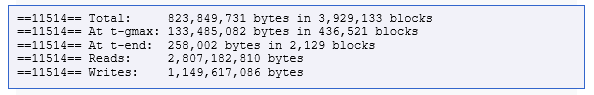
\includegraphics[width=0.8\textwidth]{DHAT.png}
  \caption{Primer izlaza alata \textit{DHAT}, izvor: \cite{DHAT}}
  \label{fig:slika2.24}
\end{figure}

Prva linija pokazuje koliko je blokova hipa i bajtova alocirano tokom celog izvršenja. Drugi red pokazuje koliko blokova i bajtova hipa je bilo živo u trenutku \textit{t-gmax}, tj.~u trenutku kada je veličina hipa dostigla svoj globalni maksimum (mereno bajtovima). Treći red pokazuje koliko je blokova i bajtova hipa bilo živo u trenutku \textit{t-end}, odnosno na kraju izvršenja. Drugim rečima, daje informaciju koliko blokova i bajtova nije izričito oslobođeno. Četvrti i peti red pokazuju koliko je bajtova unutar blokova hipa pročitano i napisano tokom čitavog izvršavanja.

Ove linije su u najboljem slučaju umerenog značaja. Korisnije informacije mogu se videti sa \textit{DHAT}-ovim prikazivačem. To omogućava činjenica da pored štampanja rezimea, \textit{DHAT} u datoteku upisuje i detaljnije informacije o profajliranju. Podrazumevano se ova datoteka naziva \texttt{dhat.out.<pid>}, gde je <pid> ID procesa programa, ali njeno ime se može promeniti pomoću opcije \texttt{--dhat-out-file}. Ova datoteka je u JSON formatu i namenjena je pregledu \textit{DHAT}-ovog pregledača. Treba imati na umu da ova datoteka može biti dosta velika u zavisnosti od veličine aplikacije. 
\textit{DHAT}-ov prikazivač se može pokrenuti u veb pregledaču učitavanjem datoteke \texttt{dh\_viev.html}. Pomoću dugmeta ''Učitaj'' (eng. \textit{load}) neophodno je odabrati \textit{DHAT} izlaznu datoteku za prikaz. Ako učitavanje traje dugo, preporučuje se ponovno pokretanje \textit{DHAT}-a sa manjom vrednošću \texttt{--num-callers} da bi se smanjile dubine steka, jer to može značajno smanjiti veličinu izlaznih datoteka \textit{DHAT}-a \cite{DHAT}. 

\subsection{BBV}
Osnovni blok je linearni presek koda sa jednom ulaznom tačkom i jednom izlaznom tačkom. Vektor osnovnog bloka (eng. \textit{basic block vector - BBV}) je lista svih osnovnih blokova unetih tokom izvršavanja programa i broj koliko je puta svaki osnovni blok pokrenut.

\textit{BBV} je alat koji generiše osnovne blok vektore za upotrebu sa alatkom za analizu \textit{SimPoint}. \textit{SimPoint} metodologija omogućava ubrzavanje arhitektonskih simulacija pokretanjem samo malog dela programa i ekstrapolacijom ukupnog ponašanja iz ovog malog dela. Većina programa pokazuje ponašanje zasnovano na fazama, što znači da će u različito vreme tokom izvršavanja program naići na vremenske intervale u kojima se k\^od ponaša slično prethodnom intervalu. Na kraju, to znači da ako možemo da detektujemo ove intervale i grupišemo ih, približna vrednost ukupnog ponašanja programa može se dobiti samo simulacijom najmanjeg broja intervala, a zatim skaliranjem rezultata. U istraživanju računarske arhitekture, pokretanje testova na simulatoru sa tačnošću ciklusa može prouzrokovati usporavanje reda veličine oko 1000 puta, što znači da su potrebni dani, nedelje ili čak duže da se izvrše kompletni  testovi. Korišćenjem \textit{SimPoint}-a ovo se može značajno smanjiti, obično za 90-95\%, uz zadržavanje razumne tačnosti.

Da bismo kreirali datoteku osnovnog vektorskog bloka, neophodno je u komandnoj liniji \textit{Valgrind}-a navesti opciju \texttt{–tool=exp-bbv}.
\begin{center}
\texttt{valgrind --tool=exp-bbv [argumenti bbva] program [argumenti programa]}
\end{center}

Podrazumevano će biti kreirana datoteka zvana \texttt{bb.out.PID}, gde je PID zamenjen ID-om procesa koji se izvršava. Ova datoteka sadrži vector osnovnog bloka. Za  programe koji se dugo izvršavaju ova datoteka može biti prilično velika, pa bi bilo pametno da je kompresujete sa \textit{gzip}-om ili nekim drugim programom za kompresiju. Da biste kreirali stvarne \textit{SimPoint} rezultate, biće vam potreban uslužni program \textit{SimPoint}, dostupan na \textit{SimPoint} veb stranici. Pod pretpostavkom da ste preuzeli \textit{SimPoint 3.2} i kompajlirali ga, kreirajte \textit{SimPoint} rezultate naredbom poput sledeće:
\begin{center}
\texttt{./SimPoint.3.2/bin/simpoint -inputVectorsGzipped \
    -loadFVFile bb.out.1234.gz \
    -k 5 -saveSimpoints results.simpts \
    -saveSimpointWeights results.weights},
\end{center}
gde je \texttt{bb.out.1234.gz} kompresovana datoteka vektora osnovnog bloka koju generiše \textit{BBV}.

Uslužni program \textit{SimPoint} vrši slučajnu linearnu projekciju pomoću 15 dimenzija, a zatim k-dimenziono grupisanje kako bi izračunao koji intervali su od interesa. U ovom primeru definisano je 5 intervala pomoću opcije -k 5.Izlazi nakon završetka rada \textit{SimPoint}-a su datoteke \texttt{results.simpts i results.weights}. Prva sadrži 5 najrelevantnijih intervala programa. Druga  sadrži težinu za skaliranje svakog intervala prilikom ekstrapolacije ponašanja u celom programu. Intervali i težine mogu se koristiti zajedno sa simulatorom koji podržava brzo premotavanje unapred. To u bukvalnom smislu znači da premotavate unapred do intervala od interesa, prikupljate statistiku za željenu dužinu intervala, a zatim koristite statistike prikupljene zajedno sa težinama za izračunavanje rezultata \cite{BBV}. 


% ------------------------------------------------------------------------------
\chapter{Regularni izrazi}
Računari su mašine koje vrše transformaciju informacija iz jednog oblika u drugi. Te infromacije se računaru predstavljaju u posebnom formatu označenim  kao podatak, a sam računar će zadatu transformaciju nad informacijama obaviti bez razumevanja značenja same informacije, kao ni transformacije koja se nad njom vrši.

U skladu sa izrečenim zaključujemo da je program specifikacija transformacije koju računar izvršava, dok je programski jezik notacija koja omogućava zapisivanje programa. Program kao specifikacija transformacije koja će biti izvršena na računaru definiše šta će program raditi, ali ne i način na koji će to uraditi. Jasno, jedan program može biti napisan različitim notacijama, odnosno različitim programskim jezicima. Uloga kompilatora jeste da transformiše tekst programa iz reprezentacije na visokom programskom jeziku (eng. \textit{high-level programming language}) u evivalentnu reprezentaciju na mašinskom jeziku, tj.~jeziku razumljivom računaru u cilju izvršavanja samog programa. U tom smislu, kompilacija se sastoji u čitanju niske karaktera koja je sastavljena u skladu sa pravilima, a sa ciljem da se generiše druga reprezentacija informacije koju ti karakteri predstavljaju.

Program napisan na nekom programskom jeziku nazivamo izvornim kodom  (eng. \textit{source code}), dok rezultat rada kompilatora nazivamo objektnim kodom (eng. \textit{object code}). Objektni k\^od može biti izražen na mašinskom jeziku, na asembleru ili na nekom drugom programskom jeziku \cite{Vitas}. 

\section{Proces kompilacije}
Transformacija teksta programa iz izvornog u objektni k\^od, koju izvršava kompilator, naziva se proces kompilacije.

Proces kompilacije obično se razlaže na dve etape:
\begin{enumerate}
\item etapa analize izvornog koda – tokom ove etape izvorni program se prevodi u odgovarajuću posrednu reprezentaciju koja prikazuje strukturu izvornog programa u obliku drveta.
\item etapa sinteze izvornog koda – tokom ove etape se koristeći rezultate iz prethodne etape na osnovu posredne reprezentacije generiše objektni k\^od.
\end{enumerate}
Svaka od etapa se kasnije deli na faze. U ovom tekstu biće detaljnije pojašnjena analiza izvornog koda, sa akcentom na regularnim izrazima, na kome ovaj rad počiva.

Tokom analize, kompilator analizira izvorni program da bi odredio njegovu strukturu i značenje. Etapa analize izvornog koda se razlaže na tri posebne faze:
\begin{enumerate}
\item leksička analiza
\item sintaksička analiza
\item semantička analiza
\end{enumerate}

Leksička analiza je faza u kojoj se karakteri iz ulazne struje karaktera rastavljaju na leksičke jedinice ili lekseme analiziranog jezika. Lekseme su minimalni, nedeljivi konstituenti jezika. Sintaksička analiza je faza u kojoj se ispituje i rekonstruiše struktura programa kao celine na osnovu niza tokena koje prosleđuje leksički analizator. Sintaksičkom analizom se utvrđuje da li je program saglasan sa gramatičkim pravilima programskog jezika, ali ne i njegova semantička konzistentnost. Opis semantike programskog jezika obično se zadaje polazeći od značenja koju pojedinačni iskazi programskog jezika vrše. Shodno tome se opis dejstva pojedinačnih iskaza nekog programskog jezika naziva semantika programskog jezika. Faza semantičke analize, koja sledi nakon sintaksičke analize, najčešće se sastoji u izvršavanju akcija koje nalaže sintaksički analizator, a koje se sastoje u kreiranju i ažuriranju informacija u tabeli simbola \cite{Vitas}.

\section{Teorija jezika}
Da bi ispitivanje izvornog koda bilo moguće, potrebno je precizno definisati izvorni jezik. Jedna klasa jezika, koja je od značaja za leksičku analizu programskih jezika, opisuje se posebnom notacijom, tj.~regularnim izrazima.

Definicija izvornog jezika mora obuhvatiti opis alfabeta ili azbuke jezika, tj.~konačan skup simbola čija je upotreba dozvoljena u jeziku, a zatim i opis svih onih niski simbola (reči) koje pripadaju tom jeziku uključujući i njihovo značenje, odnosno sintaksu i semantiku jezika. 

Neka je $\Sigma$  konačan skup. Niska (eng. \textit{string}) ili reč (eng. \textit{word}) nad $\Sigma$ je svaki konačan niz $$x = (a_1, a_2, …, a_n),$$ gde je $n \geq 0$, a $a_i \in \Sigma$ za svako $\textit{i} \in [1,n]$. Broj $n$ se naziva dužina reči i obeležava se sa $|x|$. Ako je $n=0$, reč se naziva prazna niska ili prazna reč, i obeležava se simbolom $\varepsilon$, odnosno važi $| \varepsilon |=0$.  Ako je $$y = (b_1, b_2, …, b_m)$$ neka druga reč nad $\Sigma$, tada je proizvod dopisivanja, tj.~konkatenacije reči $x$ i $y$ reč $$xy =(a_1, a_2, …, a_n, b_1, b_2, …, b_m).$$
Operacija dopisivanja je asocijativna. Skup $\Sigma$ nazivamo alfabet ili azbuka, a njegove elemente slova ili simboli.

Skup svih niski nad azbukom $\Sigma$ obeležava se sa $\Sigma^*$. Ovaj skup se naziva Klinijevo zatvorenje azbuke $\Sigma$. Na primer, ukoliko je $\Sigma = \{a,b\}$, onda je $$\Sigma^* = { \varepsilon, a, b, aa, ab, ba, bb, …}.$$
Prazna reč $\varepsilon$ je neutralni element u odnosu na dopisivanje, tj.~za $\forall x\in \Sigma, x\varepsilon = \varepsilon x = x$. Skup svih reči bez prazne reči označava se kao $\Sigma^+$, tj.~$\Sigma^+ = \Sigma^* - { \varepsilon }$. Na skupu $\Sigma^*$ nije definisan pojam inverznog elementa, tj.~ako $x \in \Sigma^+$, onda ne postoji $y \in \Sigma^+$, tdj. $xy = \varepsilon$.

Elementi azbuke $\Sigma$ se ne mogu razložiti na druge elemente, tj.~za bilo koje $a \in \Sigma$, ne postoje $b,c  \in \Sigma^+$, takvi da $a = bc$, iz čega sledi da se bilo koja reč $x \in \Sigma^*$ rastavlja na jedinstven način na elemente azbuke $\Sigma$. Imajući u vidu ova svojstva zaključujemo da je $\Sigma^*$ slobodni monoid sa skupom generatora $\Sigma$.
\begin{lem}
(Levijeva lema) Neka su $t, u, v, w \in \Sigma^*$. Ako je $tu = vw$, onda $\exists !$ reč $z  \in \Sigma^*$, tako da važi
	\begin{itemize}
	\item ili je $t = vz$ i $zu = w$
	\item ili je $v = tz$ i $zw = u.$
	\end{itemize}
\end{lem}

Neka je $v \in \Sigma^*$. Za reč $u \in \Sigma^*$ se kaže da je faktor reči $v$ ako postoje reči $v_1, v_2 \in \Sigma^*$, takve da je $v = v_1uv_2$ i to:
\begin{itemize}
\item levi faktor ili prefiks, ako je $v=uv_2$
\item desni faktor ili sufiks, ako je $v = v_1u$
\item pravi faktor ili infiks, ako je $v = v_1uv_2, v_1 \neq \varepsilon, v_2 \neq \varepsilon.$
\end{itemize}
Faktorizacija jedne reči predstavlja zapis te reči kao proizvod dopisivanja faktora. Podreč reči $v \in \Sigma^*$ je svaki podniz slova koja čine reč $v$.

\begin{defn}
(Formalni) jezik nad azbukom $\Sigma$ je bilo koji podskup skupa $\Sigma^*$: $L \subset \Sigma^*$. Ako niska $x \in L$, onda $x$ predstavlja rečenicu jezika $L$.
\end{defn}

Neka je data azbuka simbola $\Sigma = \{ a, b, c\}$. Nad ovom azbukom, neki od jezika predstavljeni su sledećim skupovima:
\begin{itemize}
\item[] $L_1 = \{a_n | n > 0\}$ – jezik koji se sastoji od niski u kojima se proizvoljan broj puta pojavljuje simbol $a$.
\item[] $L_2 = \{a_nb_m | m, n > 0\}$ – jezik koji se sastoji od niski u kojima se proizvoljan broj puta pojavljuje simbol $a$ iza čega sledi pojavljivanje simbola $b$ proizvoljan broj puta.
\end{itemize}

Jezici mogu biti konačni ili beskonačni. Konačni jezici se najjednostavnije definišu eksplicitnim navođenjem niski koje u njima predstavljaju rečenice. Problem je kako opisati na konačan način rečenice koje pripadaju jeziku koji nije konačan. Tu se dolazi do opšteg problema svakog jezika, a to je kako za datu nisku $x \in \Sigma^*$ odrediti da li je ona rečenica jezika $L$ ili ne. Najopštiju klasu algoritama koja rešava ovaj problem opisuju Tjuringove mašine. Prevelika opštost ovog mehanizma ne dozvoljava da se izrazi specifičnost koju zahtevaju programski  jezici. Uvodeći razna ograničenja, rešavanje problema pripadanja niske $x$ jeziku može se realizovati na znatno efikasniji način. Iz ugla kompilacije programskih jezika, dve klase takvih jezika su regularni jezici i kontekstno slobodni jezici.  

Pre nego što uvedemo formalnu priču o regularnim izrazima, pomenućemo neke od skupovnih operacijama koje se mogu primeniti nad jezicima. Nad jezicima se mogu izvršiti operacije unije, preseka i razlike, kao i operacija proizvoda \cite{Vitas}. 

\begin{defn}
Proizvod jezika $L_1$ i $L_2$ nad azbukom $\Sigma$ u oznaci $L_1L_2$ je jezik $$L_1L_2 = \{xy | x \in L_1, y \in L_2\}.$$
Proizvod jezika je asocijativna operacija, a {$\varepsilon$} je njen neutralni element.
\end{defn}

\begin{defn}
Za jezik $L$, $n$-ti stepen jezika $L$ je jezik: 
$$L_0 = \{ \varepsilon\} $$ 
$$L_1 = L$$
$$L_n = LL_(n-1), za  n>1.$$
\end{defn}

\begin{defn}
Iteracija ili (Klinijevo) zatvorenje jezika $L$, u oznaci $L^*$, je jezik:
$$ L^* = \bigcup_{n\geq0}L^n.$$
Pozitivno zatvorenje jezika $L$, u oznaci $L^+$, je jezik:
$$ L^+ = \bigcup_{n\geq1}L^n = L^* - \{\varepsilon\}.$$
\end{defn}

\section{Regularni izrazi i jezici}

\begin{defn}
Regularni ili racionalni izrazi nad azbukom $\Sigma$ opisuju se rekurzivno na sledeći način:
\begin{enumerate}
\item Prazan skup je regularni izraz koji se prikazuje simpolom $\emptyset$;
\item Regularni izraz $\varepsilon$ predstavlja jezik $\{\varepsilon\}$;
\item Ako je $a \in \Sigma$, onda regularni izraz $a$ predstavlja jezik $\{a\}$;
\item Ako su $p$ i $q$ regularni izrazi jezika $L(p)$ i $L(q)$, onda je:
	\begin{itemize}
	\item $(p+q)$ regularni izraz koji predstavlja jezik $L(p) \cup L(q)$.
	\item $(pq)$ regularni izraz koji predstavlja jezik $L(p)L(q)$.
	\item $(p)^*$ regularni izraz koji predstavlja jezik $(L(p))^*$.
	\item $(p)$ regularni izraz koji predstavlja jezik $L(p)$.
	\end{itemize}
\end{enumerate}
\end{defn}

Poslednje pravilo ukazuje na to da se zagrade mogu izostaviti iz regularnog izraza, a da se pritom opisani jezik ne promeni. Prilikom izostavljanja zagrada, treba znati činjenicu da su operatori *, + i konkatenacija levo asocijativni, a da im je prioritet određen sa:
\begin{center}
\textit{prioritet(*) > prioritet(konkatenacija) > prioritet(+).}
\end{center}

Operacije sa regularnim izrazima nad jezikom $\Sigma$ imaju sledeća svojstva:
\begin{itemize}
\item Operacija + je idempotentna, asocijativna i komunikativna;
\item Operacija konkatenacije je asocijativna i distributivna u odnosu na +;
\item Sledeće jednakosti važe za svaki regularni izraz:
$$\emptyset + p = p + \emptyset = p$$
$$\varepsilon p = p\varepsilon = p$$
$$\emptyset p = p\emptyset = \emptyset ;$$
\item $\emptyset^* = \varepsilon^* = \varepsilon$.
\end{itemize}

\begin{defn}
Za jedan jezik se kaže da je regularan ukoliko se može predstaviti regularnim izrazom. 
\end{defn}

Na osnovu gore navedenih svojstava regularnih izraza, skup regularnih izraza sa uvedenim operacijama predstavlja jednu algebru koju ćemo obeležiti sa $I(\Sigma)$. Važnost ove notacije ogleda se u tome što se slovo azbuke, reč koja se sastoji od tog slova, regularni izraz koji predstavlja to slovo, i na kraju jezik predstavljen regularnim izrazom beleže na isti način. 

Preslikavanje $L$ sa algebre $I(\Sigma)$ u skup regularnih izraza nad $\Sigma$ $$ L : I(\Sigma) \rightarrow P(\Sigma^*)$$ definisano je sledećim rekurzivnim pravilima:
$$ L(\emptyset) = \emptyset, L(\varepsilon) = \varepsilon, L(a) = \{a\},$$
$$ L(p+q) = L(p) \cup L(q), L(pq) = L(p)L(q), L(p^*) = L(p)^*.$$

Kažemo da je za neki regularni izraz $p$, jezik $L(p)$ jezik opisan regularnim izrazom $p$. Dva regularna izraza $p$ i $q$ su ekvivalentna, u oznaci $p \approx q$, ako opisuju isti jezik, tj.~ako važi $L(p) = L(q)$. O tome govori naredna teorema.

\begin{thm}
Za bilo koje regularne izraze $p$ i $q$ važi sledeća ekvivalencija: $$(pq)^* = \varepsilon + p(qp)^* q$$.
\end{thm}

Kao što smo se već uverili, regularni izrazi se grade polazeći od drugih regularnih izraza. To može dovesti do nepreglednosti njihovog zapisa, što rešavamo uvođenjem regularnih definicjia koje omogućuju da se određenim regularnim izrazima dodeli ime. Regularne definicije zapisujemo u obliku:
$$D_1  \rightarrow R_1$$
$$D_2  \rightarrow R_2$$
$$ ... $$
$$D_n -> R_n, $$
gde je svako $d_i$ niska nad azbukom koja je disjunktna sa azbukom $\Sigma$, različita od $d_1, d_2, …, d_{i-1}$, a svako $r_i$ regularni izraz nad azbukom $\Sigma \cup \{ d_1, d_2, …, d_{i-1}\}$.

Radi pojednostavljenja zapisivanja regularnih izraza, definicija regularnih izraza se dopunjuje dodavanjem sledećih konvencija:
\begin{itemize}
\item Neka je $r$ regularni izraz koji opisuje jezik $L(r)$. Tada je $(r)^+$ regularni izraz koji opisuje jezik $(L(r))(L(r))^*$, a $(r)?$ regularni izraz koji opisuje jezik $L(r) \cup \{\varepsilon\}$;
\item Ako su $c_1, c_2, …, c_n$ karakteri, tada se regularni izraz $c_1 + c_2 + … + c_n$ može obeležiti sa $[c_1, c_2, …, c_n]$. Izraz $[c_1-c_2]$ označava sekvencu svih karaktera $c$ tdj. $c_1 \leq c \leq c_2$.
\end{itemize}

Tako na primer slova engleske abecede označavamo sa $[A-Za-z]$, dok cifre označavamo sa $[0-9]$, itd..

Klasa jezika koji se mogu opisati regularnim izrazima je dovoljna da se opišu lekseme jednog programskog jezika. Treba imati u vidu da se složenije konstrukcije u programskom jeziku ne mogu izraziti regularnim izrazima \cite{Vitas}. 

\section{Modul re}

U današnje vreme, programski jezici imaju veoma dobru podršku za rad sa regularnim izrazima i imaju širok dijapazon upotrebe. Alat koji ovaj rad prati razvijen je u programskom jeziku Python, a \textit{re} je modul koji pruža podršku za rad sa regularnim izrazima u Python programima.

Ovaj modul pruža operacije podudaranja regularnih izraza. Važno je napomenuti da je većina operacija sa regularnim izrazima dostupna u vidu funkcija i metoda na nivou modula sa kompajliranim regularnim izrazima. Funkcije su prečice koje ne zahtevaju da prvo kompajlirate objekat regularnog izraza, ali je mana što im nedostaju neki parametri za fino podešavanje. 

Regularni izraz (ili RE) navodi niz karaktera koji mu odgovara, dok vam funkcije u ovom modulu omogućavaju da proverite da li se određeni niz karaktera poklapa sa datim regularnim izrazom (ili da li se regularni izraz podudara sa određenim nizom karaktera, što se svodi na istu stvar).
Neke od funkcija koje ovaj modul pruža, a koje su iskorišćene u alatu koji ovaj rad prati su sledeće:

\begin{itemize}
\item[$\textendash$]  \textit{re.search(pattern, string, flags=0)} - Skenira kroz \textit{string} tražeći prvu lokaciju na kojoj obrazac regularnog izraza daje podudaranje i vraća odgovarajući objekt podudaranja. Vratiće \textit{None} ako nijedna pozicija u nizu karaktera ne odgovara obrascu. Imajte na umu da se ovo razlikuje od pronalaženja podudaranja nulte dužine u nekom trenutku niza.
\item[$\textendash$]  \textit{re.match(pattern, string, flags=0)} - Ako se nula ili više znakova na početku niza karaktera \textit{string}  podudaraju sa regularnim izrazom, vratiće odgovarajući objekt podudaranja. Vratiće \textit{None} ako se niz ne podudara sa obrascem.
\item[$\textendash$]  \textit{re.split(pattern, string, maxsplit=0, flags=0)} - Podeliće nisku \textit{string} pojavljivanjima koja se poklapalu sa \textit{pattern}. 
\item[$\textendash$]  \textit{re.findall(pattern, string, flags=0)} - Vraća sva podudaranja \textit{pattern}-a u \textit{string}-u kao listu stringova, tj.~niski. Niska u kojoj se traže preklapanja - \textit{string}, skenira se s leva na desno, a poklapanja se vraćaju u redosledu u kom se i javljaju. 
\item[$\textendash$]  \textit{re.sub(pattern, repl, string, count=0, flags=0)} - Vraća string dobijen zamenom krajnjeg levog poklapanja sa \textit{pattern}-om u \textit{string}-u sa \textit{repl}. Ako poklapanje nije pronađeno, \textit{string} se vraća nepromenjen. \textit{Repl} može biti niz ili funkcija.
\end{itemize}

Kompajlirani objekti regularnog izraza podržavaju slične metode i atribute, s tim da je pozivanje istih u formi
\begin{center}
\texttt{Pattern.funkcija(argumenti).}
\end{center}

Objekti podudaranja uvek imaju logičku vrednost \textit{True}. Budući da \textit{match()} i \textit{search ()} vraćaju \textit{None} kada nema podudaranja, možete testirati da li je postojalo podudaranje jednostavnim \textit{if} izrazom. 

Objekti podudaranja podržavaju mnoge metode i atribute, a najiskorišćenija u alatu koji se razvija, a u cilju izvlačenja potrebnih informacija iz poklapanja sa regularnim izrazom je:
\begin{itemize}
\item[$\textendash$]  \textit{Match.group([group1, ...])} - Vraća jednu ili više podgrupa podudaranja. Ako postoji jedan argument, rezultat je jedan string, dok ako postoji više argumenata, rezultat je t-orka sa jednom stavkom po argumentu. Bez argumenata, \textit{group1} je  podrazumevano nula, tj.~vraća se ceo \textit{Match} objekat. Ako je indeks \textit{group} u inkluzivnom opsegu [1..99], to je string koji odgovara odgovarajućoj grupi u zagradama na toj poziciji. Ako je broj grupe negativan ili veći od broja grupa definisanih u obrascu, biće izbačen izuzetak \textit{IndexError}. Ako je grupa sadržana u delu uzorka koji se ne podudara, odgovarajući rezultat je \textit{None}. Ako je grupa sadržana u delu uzorka koji se podudarao više puta, vraća se poslednje podudaranje \cite{reModule}.
\end{itemize}

Primer korišćenja funkcije \textit{group} dat je na slici \ref{fig:slika3.1}
\begin{figure}[!ht]
  \centering
  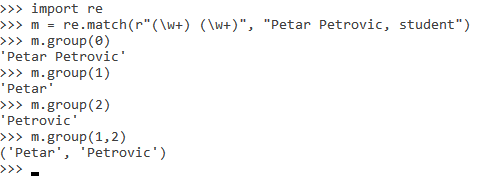
\includegraphics[width=0.7\textwidth]{reModule.png}
  \caption{Primer korišćenja funkcije \textit{group} modula \textit{re}}
  \label{fig:slika3.1}
\end{figure}

% ------------------------------------------------------------------------------

% ------------------------------------------------------------------------------
\chapter{Alat Koronka}
Alat \textit{Koronka} predstavlja alat koji automatski otkriva greske u kodu napisanom u C-u koristeci alat \textit{Valgrind}-ove distribucije \textit{Memcheck}, a zatim ih ispravlja ukoliko je to u njegovoj moći. Razvijan pod \textit{Linux} okruženjem, a implementiran u programskom jeziku \textit{Python}. Alat je nazvan \textit{Koronka}, zbog situacije u kojoj se ceo svet našao početkom 2020. godine. Osnovna svrha alata je demonstracija rada alata \textit{Valgrind}, kao i tumačenje izveštaja o greškama koje \textit{Valgrind} daje i njihovo uspešno otklanjanje. Alat je slobodno dostupan i nalazi se na linku \url{https://github.com/LMladenovic/Error_fixing_tool}. Na pomenutom linku se nalaze neophodne datoteke alata, opis sistema, kao i skup test primera i njihova pokretanja.

\section{Korišćenje alata}
Da biste pokrenuli alat \textit{Koronka} neophodno je da prethodno instalirate \textit{GCC} kompajler, sam alat \textit{Valgrind}, kao i \textit{Python}. Alat se pokreće sledećom komandom:
\begin{center}
\texttt{python koronka.py [files=[list of files]] [structures=[list of user defined structures]] c file|path to c file [other arguments] .}
\end{center}
Navedeni arumenti podrazumevaju sledeće:
\begin{itemize}
\item \texttt{files} - sadrži dodatne fajlove glavnog programa (\textit{c file}) koji se analizira (npr. \textit{.h} fajlove). Ukoliko se vаš program sastoji iz više fajlova, neophodno je da ih navedete kao argument. Bitni su iz razloga sto će \textit{Koronka} svo vreme svog rada imati niz \textit{files} u memoriji koji ce imati podatak o fajlovima nad kojima može da vrši promene. Ako se ne navede argument \textit{files}, niz \textit{files} će sadržati samo glavni program (\textit{c file}) i biće u mogućnosti da vrši promene samo nad njim.
\item \texttt{structures} - predstavlja korisnički definisane strukture u okviru programa. Kako alat podrazumevano radi samo sa primitivnim tipovima podataka, ukoliko u programu postoje korisnički definisane strukture, a ne navedu se kao argument, \textit{Koronka} neće biti u mogućnosti da ispravi greške povezane sa tim strukturama, naravno, ukoliko postoje.
\item \texttt{program args} - argumenti programa koji se analizira.
\end{itemize}

Takođe, alat \textit{Koronka} sadrži i opciju \texttt{--help } čijim će navođenjem na komandnu liniju biti ispisano uputstvo za upotrebu alata. 

Sve argumente koji se navedu prilikom pokretanja alata \textit{Koronka} obradiće funkcija za obrađivanje argumenata komandne linije i rasporediće sve podatke tamo gde treba. Nakon pokretanja alata, u direktorijumu alata će se kreirati direktorijum u formatu \textit{datum pokretanja-vreme pokretanja}. U njega će se kopirati svi podaci navedeni kao arugment \textit{files}, kao i glavni program nad kojim se vrši analiza i nad njima će biti vršene odgovarajuće promene u skladu sa otkrivenim greškama. Originalni fajlovi ostaće nepromenjeni, tamo gde su i perzistirani. Po završetku rada alata, u pomenutom direktorijumu će se naći još dva fajla. Prvi je \textit{ExecutionReport} koji sadrži detaljan izveštaj o radu alata, koje greške je našao, na koji način ih je rešio, koje fajlove, ondosno linije koda u njima je izmenio. Drugi, pod nazivom \textit{ValgrindLOG}, predstavlja izalaz alata \textit{Valgrind}, koji će se u procesu rada alata koristiti za parsiranje grešaka koje nađe alat \textit{Memcheck}. Ukoliko analizirate ispravljeni program nakon završetka rada alata alatom \textit{Memcheck}, dobićete isti izlaz koji možete videti u datoteci \textit{ValgrindLOG}. Način i logika rada alata biće opisani u sekcijama koje slede.

\section{Klasa greške}
Prilikom ispravljanja grešaka, greška koja se trenutno obrađuje biće predstavljena kao objekat klase \textit{ErrorInfo}. Na listingu \ref{lst:slika4.1} je predstavljen potpis pomenute klase.

Podaci koje klasa sadrži su sledeći:
\begin{itemize}
\item \textit{errorType} - sadrži informaciju o tipu greške, npr. nevalidno oslobađanje memorije, nedozvoljeno čitanje/pisanje itd..
\item \textit{valgrindOutput} - sadrži kompletan sadržaj sa slike \ref{fig:slika4.3}, za potrebe dodatnog parsiranja informacija o grešci.
\item \textit{files} - sadrži niz fajlova koji su povezani sa greškom, a koji bi eventualno bili ispravljeni.
\item \textit{changedFile} - sadrži ime fajla koji će biti promenjen.
\item \textit{changedLine} - sadrži tačnu liniju koda u fajlu \textit{changedFile} koja će biti promenjena.
\item \textit{problemLines} - sadrži linije u kodu koje su izazvale grešku koja se ispravlja.
\item \textit{errorReason} - sadrži razlog koji je izazvao grešku, npr. upotreba neinicijalizovane vrednosti sa steka, odnosno hipa.
\item \textit{bug} - sadrži bag u kodu, tj.~sadržaj linije koda koji je izazvao grešku.
\item \textit{bugFix} - sadrži ispravku baga, tj.~sadržaj kojim treba zameniti \textit{changedLine} da bi se greška uspešno ispravila.
\end{itemize}

\begin{lstlisting}[caption={Potpis klase \textit{ErrorInfo}}, label={lst:slika4.1},language={Python}] 
class ErrorInfo:

	# Initialisation with errorType
	def __init__(self, errorType, valgrindOutput, files):
        	self.errorType = errorType
		self.valgrindOutput = valgrindOutput
		self.files = files
		self.changedFile = ''
		self.changedLine = -1
		self.problemLines = []
		self.errorReason = []
		self.bug = ''
		self.bugFix = ''
\end{lstlisting}
%\begin{figure}[!ht]
%  \centering
%  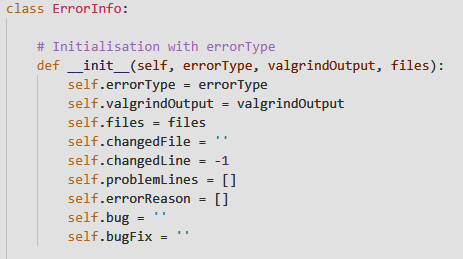
\includegraphics[width=0.7\textwidth]{ErrorClass.png}
%  \caption{Potpis klase \textit{ErrorInfo}}
%  \label{fig:slika4.1}
%\end{figure}

Za sve atribute klasa sadrži odgovarajuće \textit{get}-ere i \textit{set}-ere, kao i funkciju koja će proveravati da li je razlog greške poslat kao arument, zaista razlog koji je izazvao grešku koja se obrađuje. Prikaz funkcije dat je na listingu \ref{lst:slika4.2}.

\begin{lstlisting}[caption={Prikaz funkcije koja proverava validnost razloga greške}, label={lst:slika4.2},language={Python}] 
def isKnownReason(self, newReason):
	for reason in self.errorReason:
		if reason.find(newReason) >= 0:
			return True
			break
	return False
\end{lstlisting}

%\begin{figure}[!ht]
%  \centering
%  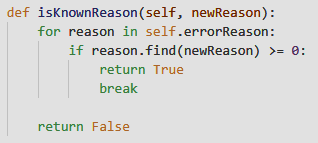
\includegraphics[width=0.7\textwidth]{ErrorReason.png}
%  \caption{Prikaz funkcije koja proverava validnost razloga greške}
%  \label{fig:slika4.2}
%\end{figure}

Na slici \ref{fig:slika4.3} prikazan je segment izveštaja alata \textit{Valgrind} koji predstavlja jednu grešku koju treba ispraviti. Žutom bojom je obeležen deo koji predstavlja tip greške, zelenom bojom deo koji predstavlja razlog greške, dok su plavom bojom obeležene sumnjive(problematične) linije. Ti podaci će redom biti smešteni u \textit{errorType}, \textit{errorReason} i \textit{problemLines}. Sve potrebne informacije od značaja iz datog iz datog segmenta izveštaja dobićemo upotrebom regularnih izraza.

\begin{figure}[!ht]
  \centering
  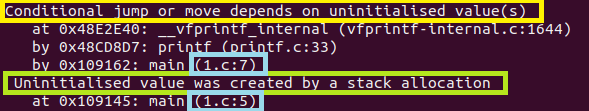
\includegraphics[width=0.7\textwidth]{ErrorClassExplaination.png}
  \caption{Prikaz izveštaja za jednu grešku}
  \label{fig:slika4.3}
\end{figure}

Na osnovu \textit{errorType} i \textit{errorReason} biće određeno koji će šablon biti upotrebljen za ispravljanje greške. Na osnovu \textit{problemLines} biće pronađena tačna linija koda koja je izazvala grešku, a iz nje izvučeni podaci koji su neophodni za ispravljanje greške, kao i iz ostalih linija ukoliko sadrže informacije od značaja. Kada se neophodni podaci o grešci izvuku i nađe njeno rešenje, biće postavljene vrednosti \textit{changedFile}, \textit{changedLine}, \textit{bug}, \textit{bugFix}. Kada se obezbede svi podaci, dalje izvršavanje alata prepušta se sistemu za praćenje istorije promena koji je opisan u \ref{istorija}.

\section{Mehanizam praćenja istorije}\label{istorija}
Sve promene koje je alat \textit{Коronka} izvršio nad fajlovima biće praćene pomoću mehanizma za praćenje istorije. Svaka promena biće sačuvana pojedinačno u nizu \textit{history} u vidu uređene trojke \textit{(izmena u kodu, promenjena linja koda, fajl nad kojim se vrši promena)}. Ovakav vid praćenja istorije je dobar iz više razloga. Na primer, može se desiti da imamo istu liniju koda koja izaziva grešku koja se nalazi u dva različita fajla. Promena tih linija bez praćenja fajla nad kojim se vrši promena neće biti moguća u oba fajla, kako je ispravka greške opet ista linija koda sa određenim dodacima. Takođe, može se desiti na primer da u istom fajlu imamo dva bloka unutar kojih postoji linija koja izaziva problem. To su dakle dve greške, čije će rešenje biti dve potupuno iste linije koda, izmenjene u dve različite linije koda u istom fajlu. Ukoliko mehanizam praćenja istorije ne pamti i liniju koda u kojoj su promene izvršene, to neće biti moguće.  

Prilikom pokretanja alata niz \textit{history} sadrži samo jednu trojku, tj.~\textit{(' ', -1, ' ')}. Kako se greške iterativno ispravljaju, svaka iteracija predstavlja pokušaj alata da datu grešku ispravi, što je bliže opisano u sekciji \ref{algoritam}. Za mehanizam praćenja istorije je to važno jer će on biti taj koji će validirati trenutni predlog za ispravku greške koje je alat našao. Prvi slučaj je da se predlog ispravke ne nalazi u istoriji, on će biti implementiran i dodat isoriji izmena u nadi da će se greška uspešno ispraviti. U drugom slučaju, predlog ispravke se već nalazi u istoriji izmena, što je signal alatu da je predlog rešenja već implementiran i da ta implementacija nije ispravila grešku, te da alat nastavi sa traženjem optimalnog rešenja. U teoriji, ukoliko alat iskoristi sve mehanizme za ispravljanje određene greške koje poseduje, tj.~implementira sve predloge rešenja koje je u mogućnosti da predloži, a greška ostane neispravljena, alat će nastaviti sa radom i pokušati da ispravi ostale greške, ukoliko postoje, a navedena greška će ostati neispravljena, a korisnik će biti obavešten da postoji greška koja nažalost nije ispravljena. Jasno, prilikom nalaženja rešenja koje će biti zaista i biti implementirano, to rešenje biva dodato u istoriju, a alat nastavlja sa iteracijama ispravljanja ostalih grešaka.

\section{Algoritam izvršavanja}\label{algoritam}
Kao što je već rečeno, pri pokretanju alata generiše se odgovarajući direktorijum, u njega se kopiraju svi navedeni (potrebni) fajlovi, formiraju se nizovi \textit{structures}, \textit{files} i \textit{history}. Nakon početnih podešavanja sledi iterativno kompilacija programa i analiza \textit{Valgrind}-ovim alatom \textit{Memcheck} čiji izlaz se smešta u datoteku \textit{ValgrindLOG.txt}. Ovaj fajl se parsira, i iz njega se čitaju informacije o greškama iterativno. Kad alat naiđe na gresku, parsira je, nakon čega proba da je ispravi ukoliko je u mogućnosti. Ukoliko nađe resenje koje već nije primenjeno, biće implementirano nakon čega alat ide u novu iteraciju kompilacije i provere grešaka, uz prethodno ažuriranje istorije i izveštaja o ispravljenim greškama. Proces se ponavlja dokle god ima grešaka koje nisu ispravljene, a koje je \textit{Koronka} u mogućnosti da ispravi. Grafički prikaz algoritma dat je na slici \ref{fig:slika4.4}.

\begin{figure}[!ht]
  \centering
  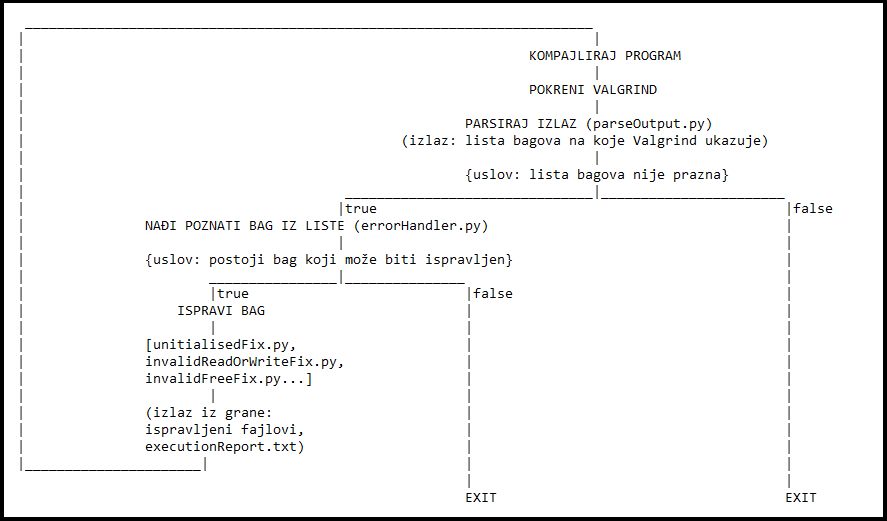
\includegraphics[width=0.9\textwidth]{ExecutingAlgorithm.png}
  \caption{Algoritam izvršavanja alata \textit{Koronka}}
  \label{fig:slika4.4}
\end{figure}

\section{Šabloni za ispravljanje grešaka}
Alat \textit{Koronka} sadrži nekoliko šablona od kojih svaki ispravlja određenu vrstu grešaka. Šablon koji će biti primenjen za ispravljanje date greške određen je vrstom greške kao i razlogom koji je datu grešku izazvao, što znači da su šabloni ekskluzivno mapirani tipom i razlogom greške. Bez obzira na optimizaciju koji \textit{Memcheck} poseduje za ispisivanje izveštaja o grešci, i dalje ispisuje par paragrafa koji se odnose na istu grešku, sa različitim razlogom, odnosno tipom (pogledati npr. sliku \ref{fig:slika2.7}). Razlog tome je taj što \textit{Memcheck} prati izvršavanje od početka, odnosno prati indirektan put te greške. To dalje znači da ne moramo da mapiramo sve tipove i razloge grešaka, već samo one koje će nam dati dovoljno informacija za ispravljanje greške. Kada ispravimo grešku, iz izveštaja koji je sadržao par paragrafa za istu, nestaće svi paragrafi kako je greška otklonjena, a za njeno otklanjanje smo koristili samo neophodnu količinu podataka, a ne sve podatke koje smo imali. Na taj način doprinosimo efikasnosti alata. Šabloni su smešteni u fajlove sa sufiksom \textit{Fix}, dok u imenu sadrže i tip greške koji ispravljaju. 

Kao što je već rečeno, šabloni su orijentisani prvenstveno prema tipu greške koju ispravljaju, pa će njihovo izlaganje biti realizovano kroz tipove grešaka koje ispravljaju. 

\subsection{Korišćenje neinicijalizovane vrednosti}
Šablon koji ispravlja ovaj tip grešaka mapiran je tipom \textit{''Conditional jump or move depends on uninitialised value(s)''}, dok razlozi za grešku mogu biti \textit{''Uninitialised value was created by a stack allocation''} i \textit{''Uninitialised value was created by a heap allocation''}, u zavisnosti od toga da li je reč o statičkoj, odnosno dinamički alociranoj memoriji. Ispis alata \textit{Valgrind} koji dobijamo za ovaj tip greške u slučaju statičke memorije, a na osnovu kog je ispravljamo, dat je na slici \ref{fig:slika4.5}.

\begin{figure}[!ht]
  \centering
  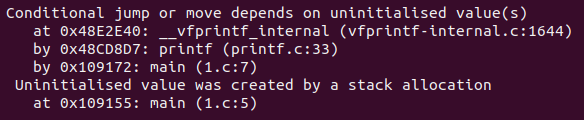
\includegraphics[width=0.9\textwidth]{UninitialisedStatic.png}
  \caption{Ispis greške korišćenja statičke neinicijalizovane promenljive}
  \label{fig:slika4.5}
\end{figure}

Iz datog izveštaja dobijamo informacije od važnosti za ispravljanje greške kao što su linije koda u kojima se koristi neinicijalizovana promenljiva, kao i liniju koda i fajl u kom počinje blok u kom je ta promenljiva definisana. Kako nemamo tačnu liniju koda u kojoj je promenljiva definisana, već blok, grešku ćemo ispraviti inicijalizovanjem svih neinicijalizovanih vrednosti u okviru tog bloka. 

Analizom linija koda datog bloka poklapanjem sa regularnim izrazom $ ([ \\t]*)([a-zA-Z_-]+)[ ]+([a-zA-Z_-]+).*; $ dobijamo liniju koda gde imamo neinicijalizovanu definisanu promenljivu. Ona može biti i višedimenziona, pa pre inicijalizacije vršimo i tu proveru da bi je, ukoliko je to slučaj, adekvatno inicijalizovali. Iz rezultata dobijenih poklapanjem sa regularnim izrazima izvlačimo podatke poput tipa promenljive, imena, a u slučaju višedimenzionog niza još i dimenzije. Za inicijalizaciju promenljivih koristimo funkciju prikazanu na listingu \ref{lst:slika4.6}, dok u slučaju nizova, odnosno višedimenzionih nizova, koristimo pomoćnu funkciju koja koristi petlje za inicijalizaciju, a koja se suštinski oslanja na funkciju sa listinga \ref{lst:slika4.6}.

\begin{lstlisting}[caption={Funkcija inicijalizacije}, label={lst:slika4.6},language={Python}] 
def initialise(varType):
	initialisator = {
		'int': '0',
		'double': '0',
		'float': '0',
		'boolean': 'False',
		'char': '\'\\0\'',
		'short': '0',
		'long': '0'
	    }
	
	if varType in initialisator:
		return initialisator[varType]
	else:
		return 'Invalid'
\end{lstlisting}

%\begin{figure}[!ht]
%  \centering
%  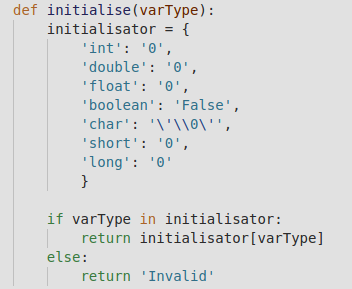
\includegraphics[width=0.5\textwidth]{InitialisationFunction.png}
%  \caption{Funkcija inicijalizacije}
%  \label{fig:slika4.6}
%\end{figure} 

U slučaju da je neinicijalizovana promenljiva korisnički definisana struktura, ukoliko je ona navedena kao argument komandne linije, alat će biti u mogućnosti da ispravi ovu grešku. Ispravljanje se sastoji u tome što će alat pronaći kako je ta struktura definisana, odnosno koji su njeni činioci. Koristeći odgovarajuću funkciju iz \textit{userDefinedStructuresHandler}-a, u kome su definisane sve operacije nad korisnčkim strukturama, inicijalizovaće celu strukturu, redom, inicijalizujući njene činioce, indirektno koristeći funkciju sa listinga \ref{lst:slika4.6}. Takođe, podržana je i inicijalizacija nizova, odnosno višedimenzionih nizova korisničkih struktura. 

Nakon što smo opisali mehanizam inicijalizacije, ispravku greške formiramo tako što zamenimo problematičnu liniju koda linijom gde je promenljiva definisana i inicijalizovana, dok u slučaju nizova i višedimenzionih nizova, problematičnu liniju menjamo blokom koda koji se sastoji iz definicije promenljive nakon koje sledi inicijalizacija korišćenjem petlje, odnosno petlji u slučaju višedimenzionih nizova. 

Ispis alata \textit{Valgrind} koji dobijamo za ovaj tip greške u slučaju dinamički alocijrane memorije, tj.~upotrebe pokazivača, a na osnovu kog je ispravljamo, dat je na slici \ref{fig:slika4.7}.

\begin{figure}[!ht]
  \centering
  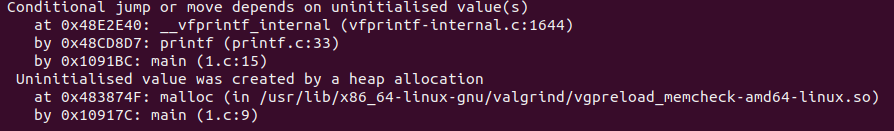
\includegraphics[width=0.9\textwidth]{UninitialisedDinamic.png}
  \caption{Ispis greške korišćenja dinamiči alocirane neinicijalizovane promenljive (pokazivača)}
  \label{fig:slika4.7}
\end{figure} 

Za razliku od greške upotrebe neinicijalizovane promenljive koja je statički definisana, ovde, u izveštaju pored linija koda u kojima se koristi ta promenljiva dobijamo i informaciju o tačnoj liniji koda i fajlu u kom je promenljiva definisana. Način inicijalizacije je isti kao kod statički definisanih promenljivih, dok potrebne informacije dobijamo primenom nešto izmenjenim regularnim izrazima. Takođe, ukoliko je promenljiva samo pokazivač, bez alokacije memorije prilikom definicije iste, njena vrednost biće postavljena na \textit{NULL}. Regularni izraz koji koristimo u ovom slučaju jeste $ (malloc|calloc|realloc)(.+); $, dok se preciznije dobijanje informacije o grešci dobija specijalizacijom pomenutog izraza. Na osnovu rezultata primene pomenutih regularnih izraza dobijamo informacije o tipu pokazivača, imena pokazivača kao i veličini alocirane memorije. Takođe, i u ovom slučaju imamo podršku za rad sa korisnički definisanim strukturama. 

Nakon sakupljanja potrebnih informacija ispravku greške formiramo na isti način kao i kod statiči definisanih promenljivih, tj.~problematičnu liniju menjamo blokom koji pored te linije sadrži i k\^od koji vrši inicijalizaciju, indirektno naslonjen na funkciju sa listinga \ref{lst:slika4.6} i inicijalizacione funkcije koje koriste petlje.

\subsection{Nevalidno čitanje/pisanje}
Ovakav tip grešaka mapiran je tipom greške \textit{''Invalid read of size x''} u slučaju nevalidnog čitanja, odnosno \textit{''Invalid write of size x''} u slučaju nevalidnog pisanja, gde je \textit{x} broj bajtova. Razlog greške kojim se ova greška mapira je \textit{''Address adr is y bytes after a block of size z alloc'd''} u slučaju prekoračenja s desne strane, odnosno \textit{''Address adr is y bytes before a block of size z alloc'd''} u slučaju prekoračenja s leve strane, gde \textit{adr} predstavlja heksadekadni zapis adrese, a \textit{y} i \textit{z} broj bajtova. To se jasno može videti na slici \ref{fig:slika4.8}.

\begin{figure}[!ht]
  \centering
  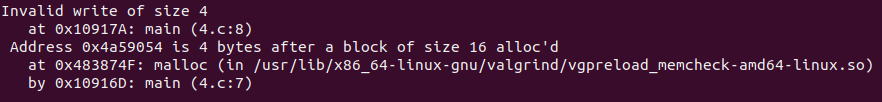
\includegraphics[width=0.9\textwidth]{InvalidReadErrorExample.png}
  \caption{Ispis greške nevalidnog čitanja}
  \label{fig:slika4.8}
\end{figure} 

Analizom segmenta sa slike \ref{fig:slika4.8}, odnosno samo razloga i tipa greške, možemo da dobijemo informaciju koliko je velika memorija kojoj pokušavamo da pristupimo, ili da je izmenimo, a koja nije alocirana. Ispravka bi bila da memoriju koju program alocira, a sa kojom je pokušana interakcija, proširimo za vrednost koju dobijamo primenom pomenutih informacija. Takođe, na slici \ref{fig:slika4.8} vidimo da dobijamo i tačnu liniju koda, odnosno fajl gde je memorija alocirana. Baš tu liniju koda menjamo ispravnom, a ispravka se sastoji u tome da pogrešnu veličinu memorije koja se alocira zamenimo ispravnom, uvećanom za broj bitova koji dobijemo analizom greške. Na ovaj način ispravljamo greške koje su povezane sa prekoračenjem s desne strane. U slučaju prekoračenja s leve strane, pristupamo memoriji kojoj nam nije dozvoljeno, odnosno arument pristupa je vrednost manja od 0, kako znamo da indeksi pristupa alociranoj memoriji kreću od 0. Ovu grešku ispravljamo tako što pogrešan indeks pristupa zamenimo njegovom apsolutnom vrednošću i na taj način ispravni indeksi ostaju takvi, dok pogrešne stavljamo u interval ispravnih. U slučaju da apsolutna vrednost pomenutog indeksa izaziva grešku prekoračenja s desne strane, memorija će biti proširena, odnosno ispravljaće se greška nevalidnog čitanja/pisanja u slučaju prekoračenja s desne strane.  


\subsection{Nevalidno oslobađanje memorije}
Ovakav tip grešaka mapiran je tipom greške \textit{''Invalid free() / delete / delete[] / realloc()''}. Za ovaj tip greške razlog nije od presudnog značaja, tako da se mapiranje vrši samo nad tipom greške. Na slici \ref{fig:slika4.9} prikazan je segment ispisa greške koji koristimo da bismo je ispravili. Analizom ispisa sa slike dobijamo preciznu informaciju o liniji koda, kao i o fajlu gde je izvršeno nevalidno oslobađanje memorije. Ovu grešku ispravljamo tako što tu liniju izbrišemo, odnosno otklonimo nevalidno oslobađanje memorije. 

\begin{figure}[!ht]
  \centering
  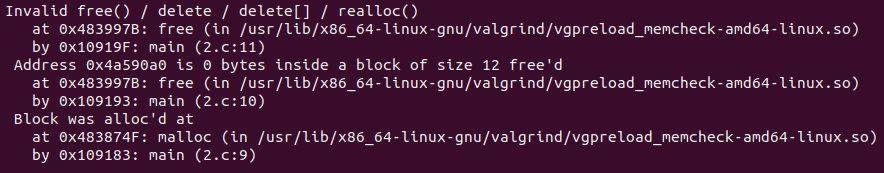
\includegraphics[width=0.9\textwidth]{InvalidFreeErrorPartOfResume.png}
  \caption{Ispis greške nevalidnog oslobađanja memorije}
  \label{fig:slika4.9}
\end{figure} 

\subsection{Sumnjive vrednosti argumenata}
Ovakav tip grešaka mapiran je tipom greške \textit{'' Argument 'size' of function x has a fishy (possibly negative) value: y''}, gde je \textit{x} naziv funkcije, a \textit{y} vrednost argumenta. Za ovaj tip greške mapiranje se vrši samo nad tipom greške, kako je sam razlog nedozvoljena vrednost argumenta, što \textit{Memcheck} ispisuje u okviru tipa greške. Na slici \ref{fig:slika4.10} prikazan je ispis greške koji koristimo da bismo je ispravili. Analizom ispisa sa slike dobijamo preciznu informaciju o liniji koda, kao i o fajlu gde gde je pozvana funkcija koja sadrži sumnjivi arugment. U zavisnosti od funkcije, primenom adekvatnog regularnog izraza nalazimo mesto gde je sumnjivi arugment, i isti menjamo njegovom apsolutnom vrednošću, da bi dobili ispravnu vrednost argumenta. Dakle, ovu grešku ispravljamo tako što izmenimo sumnjivi argument u pozivu funkcije u okviru problematične linije ispravnim, odnosno računamo apsolutnu vrednost sumnjivog argumenta. 

\begin{figure}[!ht]
  \centering
  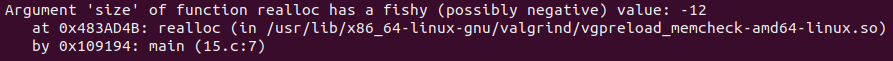
\includegraphics[width=0.9\textwidth]{reallocFishyArgument.png}
  \caption{Ispis greške sumnjive vrednosti argumenta}
  \label{fig:slika4.10}
\end{figure} 

\section{Primer rada alata}
Analiza i ispravka programa sa listinga \ref{lst:slika2.4} predstavljena je u ovoj sekciji. Dati program sadrži grešku upotrebe neinicijalizovane promenljive koja će biti ispravljena. Alat pokrećemo komandom u komandnoj liniji:
\begin{center}
\textit{python koronka.py program.c}.
\end{center}

Izgled komandne linije nakon pokretanja alata prikazan je na slici \ref{fig:slika4.11}. 
\begin{figure}[!ht]
  \centering
  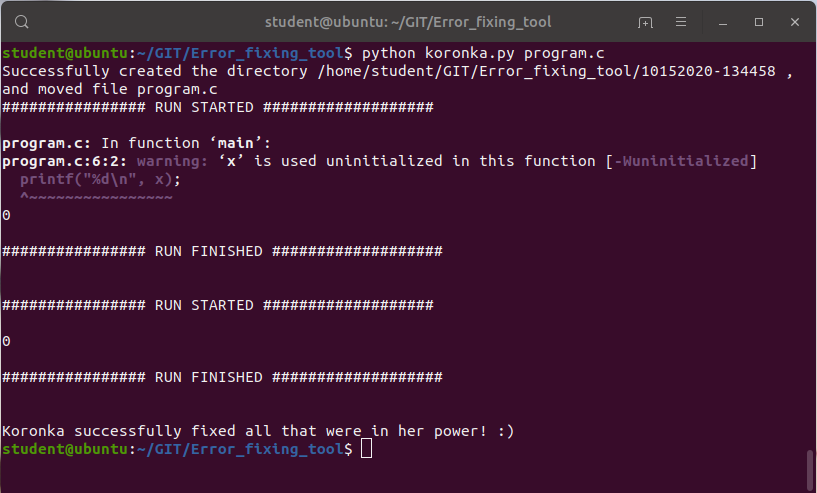
\includegraphics[width=0.6\textwidth]{TerminalOutput.png}
  \caption{Izgled terminala nakon izvršavanja alata \textit{Koronka}}
  \label{fig:slika4.11}
\end{figure}

Direktorijum koji je formiran i dodeljen ovom konkretnom pokretanju alata i njegovom izvršavanju prikazan je na slici \ref{fig:slika4.12}, dok su izmenjen program nakon izvršavanja alata \textit{Koronka}, kao i izveštaj, prikazani na slikama \ref{fig:slika4.13} i \ref{fig:slika4.14}.
\begin{figure}[!ht]
  \centering
  
\includegraphics[width=0.6\textwidth]{DateTimeFolder.png}
  \caption{Izgled foldera u formatu \textit{datum pokretanja - vreme pokretanja} koji formira alat \textit{Koronka}}
  \label{fig:slika4.12}
\end{figure}

\begin{figure}[!ht]
  \centering
  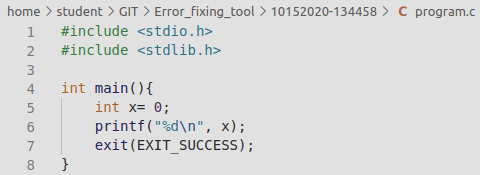
\includegraphics[width=0.6\textwidth]{FixedProgram.png}
  \caption{Izgled ispravljenog programa alatom \textit{Koronka}}
  \label{fig:slika4.13}
\end{figure}

\begin{figure}[!ht]
  \centering
  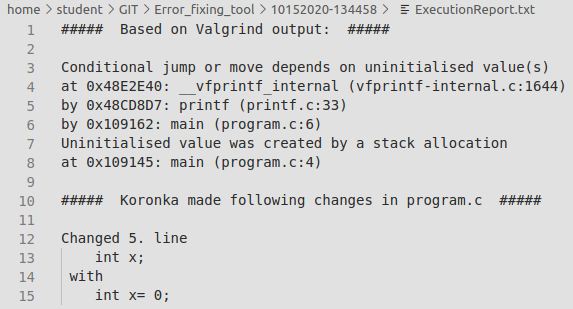
\includegraphics[width=0.6\textwidth]{ExecutionReport.png}
  \caption{Izgled izveštaja nakon izvršavanja alata \textit{Koronka}}
  \label{fig:slika4.14}
\end{figure}

Prikazani primer deo je skupa test primera nalazi se u direktorijumu \textit{Example} u okviru glavnog direktorijuma alata. Podeljeni su po folderima, a takođe se mogu i naći pokretanja i ispravke koje je \textit{Koronka} implementirala nad tim test primerima. Skup test primera dostupan je na linku \url{https://github.com/LMladenovic/Error_fixing_tool/tree/master/Example}. 

% ------------------------------------------------------------------------------

% ------------------------------------------------------------------------------
\chapter{Zaključak}
Analiza i otkrivanje grešaka koje možemo otkriti alatima iz distribucije \textit{Valgrind} ručno obično može biti mukotrpan i ne tako retko neefikasan postupak kad su u pitanju veliki programi. Srećom, alat \textit{Valgrind} je tu da pomogne u prevazilaženju tog problema. Alat \textit{Memcheck} otkriva greške u radu sa memorijom koje mogu da dovedu do pada programa, a koje kompilator nije u mogućnosti da otkrije, a koji zauzima centralno mesto ovog rada. Ostali alati \textit{Valgrind} distribucije mogu da otkriju druge probleme, poput grešaka u radu sa nitima i sl., čijom detekcijom i ispravljanjem možete doprineti performansama i boljem radu softvera koji razvijate. Princip funkcionisanja ovih alata, a pre svega alata \textit{Memcheck}, obrađeno je u ovom radu. 

Nakon što analizom programa nekim od alata distibucije \textit{Valgrind} detektujemo greške, ukoliko postoje, neophodno je da razumemo izlaz koji nam je alat dao, i da na osnovu njega pokušamo da popravimo greške. Alat koji je iznet u ovom radu pokušava da taj proces automatizuje, odnosno da razume izlaz koji je alat \textit{Memcheck} dao, i da na osnovu njega korišćenjem adekvatnih šablona ispravi otkrivene greške. Pokriven je širok dijapazon grešaka, što ne isključuje da postoje greške koje mogu biti otkrivene daljim razvojem, a koje alat \textit{Koronka} ne pokriva. 

Što se daljeg razvoja alta tiče, mogu se dodatno specijalizovati i unaprediti postojeći mehanizmi i šabloni. Kako struktura alata liči na mikro servis, alat se može iskoristiti kao deo nekog novog alata, ili kao odvojeni deo skupa alata. Takođe, može biti proširen dijapazon grešaka koji alat ispravlja korišćenjem ostalih alata distribucije \textit{Valgrind} za otkrivanje istih. 
% ------------------------------------------------------------------------------

% ------------------------------------------------------------------------------
% Literatura
% ------------------------------------------------------------------------------
\literatura

% ==============================================================================
% Završni deo teze i prilozi
\backmatter
% ==============================================================================

% ------------------------------------------------------------------------------
% Biografija kandidata
\begin{biografija}
  \textbf{Lazar Mladenović} rođen je 24.02.1996. u Leskovcu. Osnovnu školu završio je 2010. u Leskovcu, kao đak generacije i nosilac Vukove diplome. U tom periodu biva zainteresovan za programiranje, pa se može reći da mu je to odredilo dalji tok obrazovanja. Prirodno-matematički smer leskovačke Gimnazije završava 2014., takođe kao nosilac Vukove diplome.
  
  2014. upisuje Matematički fakultet u Beogradu, smer Primenjena matematika, da bi se  dve godine kasnije prebacio na smer Računarstvo i informatika. Isti završava 2019. godine. Nakon diplomiranja upisuje master studije na istom smeru i fakultetu. 
  
  Oblasti interesovanja uključuju pre svega razvoj i verifikaciju softvera, kao i primenu programiranja u auto industriji.  
    
\end{biografija}
% ------------------------------------------------------------------------------

\end{document}
